\begin{figure}[H] \centering % Created by tikzDevice version 0.12.4 on 2023-08-13 18:11:18
% !TEX encoding = UTF-8 Unicode
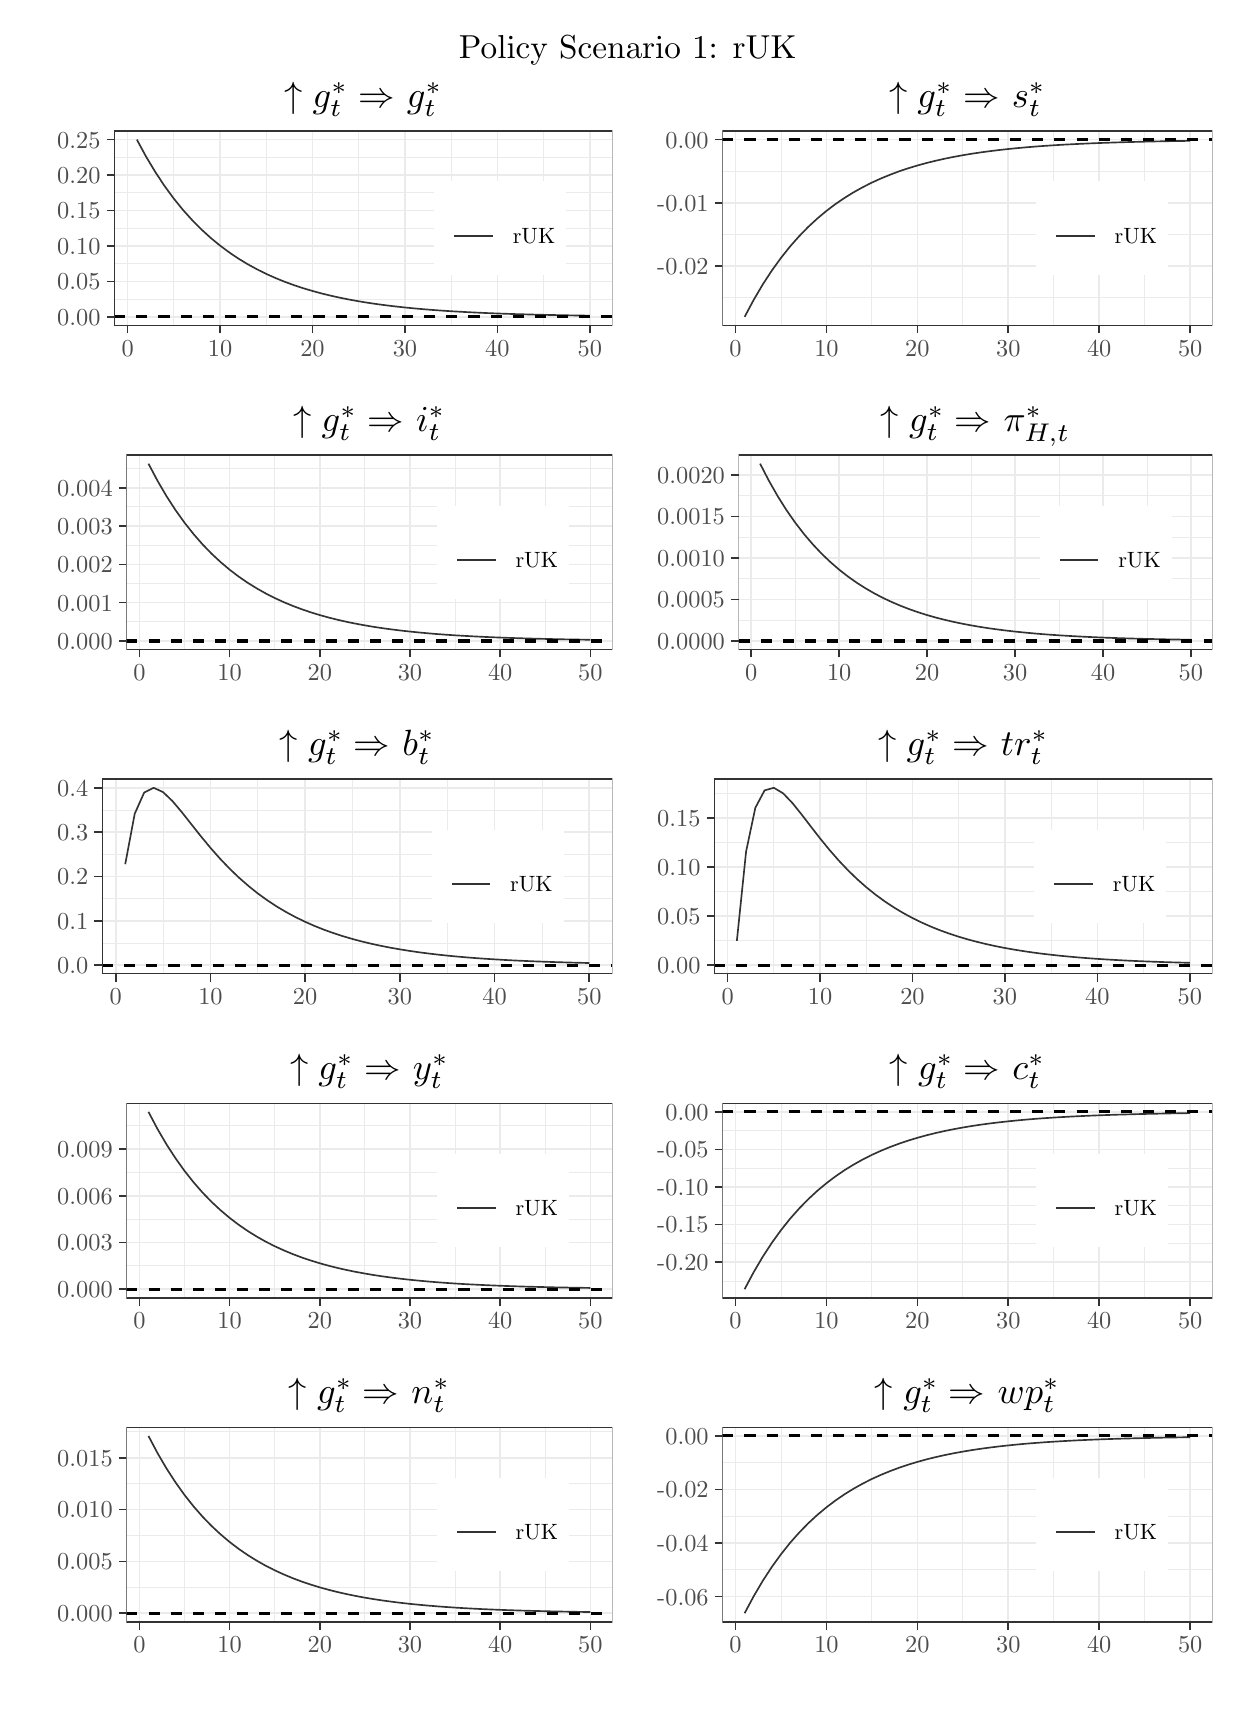
\begin{tikzpicture}[x=1pt,y=1pt]
\definecolor{fillColor}{RGB}{255,255,255}
\path[use as bounding box,fill=fillColor,fill opacity=0.00] (0,0) rectangle (433.62,599.84);
\begin{scope}
\path[clip] (  0.00,468.44) rectangle (216.81,585.55);
\definecolor{drawColor}{RGB}{255,255,255}
\definecolor{fillColor}{RGB}{255,255,255}

\path[draw=drawColor,line width= 0.6pt,line join=round,line cap=round,fill=fillColor] (  0.00,468.44) rectangle (216.81,585.55);
\end{scope}
\begin{scope}
\path[clip] ( 31.27,492.12) rectangle (211.31,562.59);
\definecolor{fillColor}{RGB}{255,255,255}

\path[fill=fillColor] ( 31.27,492.12) rectangle (211.31,562.59);
\definecolor{drawColor}{gray}{0.92}

\path[draw=drawColor,line width= 0.3pt,line join=round] ( 31.27,501.73) --
	(211.31,501.73);

\path[draw=drawColor,line width= 0.3pt,line join=round] ( 31.27,514.54) --
	(211.31,514.54);

\path[draw=drawColor,line width= 0.3pt,line join=round] ( 31.27,527.36) --
	(211.31,527.36);

\path[draw=drawColor,line width= 0.3pt,line join=round] ( 31.27,540.17) --
	(211.31,540.17);

\path[draw=drawColor,line width= 0.3pt,line join=round] ( 31.27,552.98) --
	(211.31,552.98);

\path[draw=drawColor,line width= 0.3pt,line join=round] ( 52.81,492.12) --
	( 52.81,562.59);

\path[draw=drawColor,line width= 0.3pt,line join=round] ( 86.22,492.12) --
	( 86.22,562.59);

\path[draw=drawColor,line width= 0.3pt,line join=round] (119.62,492.12) --
	(119.62,562.59);

\path[draw=drawColor,line width= 0.3pt,line join=round] (153.02,492.12) --
	(153.02,562.59);

\path[draw=drawColor,line width= 0.3pt,line join=round] (186.43,492.12) --
	(186.43,562.59);

\path[draw=drawColor,line width= 0.6pt,line join=round] ( 31.27,495.32) --
	(211.31,495.32);

\path[draw=drawColor,line width= 0.6pt,line join=round] ( 31.27,508.14) --
	(211.31,508.14);

\path[draw=drawColor,line width= 0.6pt,line join=round] ( 31.27,520.95) --
	(211.31,520.95);

\path[draw=drawColor,line width= 0.6pt,line join=round] ( 31.27,533.76) --
	(211.31,533.76);

\path[draw=drawColor,line width= 0.6pt,line join=round] ( 31.27,546.58) --
	(211.31,546.58);

\path[draw=drawColor,line width= 0.6pt,line join=round] ( 31.27,559.39) --
	(211.31,559.39);

\path[draw=drawColor,line width= 0.6pt,line join=round] ( 36.11,492.12) --
	( 36.11,562.59);

\path[draw=drawColor,line width= 0.6pt,line join=round] ( 69.52,492.12) --
	( 69.52,562.59);

\path[draw=drawColor,line width= 0.6pt,line join=round] (102.92,492.12) --
	(102.92,562.59);

\path[draw=drawColor,line width= 0.6pt,line join=round] (136.32,492.12) --
	(136.32,562.59);

\path[draw=drawColor,line width= 0.6pt,line join=round] (169.72,492.12) --
	(169.72,562.59);

\path[draw=drawColor,line width= 0.6pt,line join=round] (203.13,492.12) --
	(203.13,562.59);
\definecolor{drawColor}{gray}{0.20}

\path[draw=drawColor,line width= 0.6pt,line join=round] ( 39.45,559.39) --
	( 42.79,553.22) --
	( 46.13,547.65) --
	( 49.47,542.61) --
	( 52.81,538.06) --
	( 56.15,533.94) --
	( 59.50,530.23) --
	( 62.84,526.87) --
	( 66.18,523.83) --
	( 69.52,521.09) --
	( 72.86,518.61) --
	( 76.20,516.36) --
	( 79.54,514.34) --
	( 82.88,512.51) --
	( 86.22,510.85) --
	( 89.56,509.36) --
	( 92.90,508.01) --
	( 96.24,506.79) --
	( 99.58,505.68) --
	(102.92,504.69) --
	(106.26,503.78) --
	(109.60,502.97) --
	(112.94,502.23) --
	(116.28,501.57) --
	(119.62,500.97) --
	(122.96,500.42) --
	(126.30,499.93) --
	(129.64,499.49) --
	(132.98,499.09) --
	(136.32,498.73) --
	(139.66,498.40) --
	(143.00,498.10) --
	(146.34,497.83) --
	(149.68,497.59) --
	(153.02,497.37) --
	(156.36,497.18) --
	(159.70,497.00) --
	(163.04,496.84) --
	(166.38,496.69) --
	(169.72,496.56) --
	(173.06,496.44) --
	(176.40,496.33) --
	(179.74,496.24) --
	(183.08,496.15) --
	(186.43,496.07) --
	(189.77,496.00) --
	(193.11,495.93) --
	(196.45,495.87) --
	(199.79,495.82) --
	(203.13,495.77);
\definecolor{drawColor}{RGB}{0,0,0}

\path[draw=drawColor,line width= 1.1pt,dash pattern=on 4pt off 4pt ,line join=round] ( 31.27,495.32) -- (211.31,495.32);
\definecolor{drawColor}{gray}{0.20}

\path[draw=drawColor,line width= 0.6pt,line join=round,line cap=round] ( 31.27,492.12) rectangle (211.31,562.59);
\end{scope}
\begin{scope}
\path[clip] (  0.00,  0.00) rectangle (433.62,599.84);
\definecolor{drawColor}{gray}{0.30}

\node[text=drawColor,anchor=base east,inner sep=0pt, outer sep=0pt, scale=  0.88] at ( 26.32,492.29) {0.00};

\node[text=drawColor,anchor=base east,inner sep=0pt, outer sep=0pt, scale=  0.88] at ( 26.32,505.11) {0.05};

\node[text=drawColor,anchor=base east,inner sep=0pt, outer sep=0pt, scale=  0.88] at ( 26.32,517.92) {0.10};

\node[text=drawColor,anchor=base east,inner sep=0pt, outer sep=0pt, scale=  0.88] at ( 26.32,530.73) {0.15};

\node[text=drawColor,anchor=base east,inner sep=0pt, outer sep=0pt, scale=  0.88] at ( 26.32,543.55) {0.20};

\node[text=drawColor,anchor=base east,inner sep=0pt, outer sep=0pt, scale=  0.88] at ( 26.32,556.36) {0.25};
\end{scope}
\begin{scope}
\path[clip] (  0.00,  0.00) rectangle (433.62,599.84);
\definecolor{drawColor}{gray}{0.20}

\path[draw=drawColor,line width= 0.6pt,line join=round] ( 28.52,495.32) --
	( 31.27,495.32);

\path[draw=drawColor,line width= 0.6pt,line join=round] ( 28.52,508.14) --
	( 31.27,508.14);

\path[draw=drawColor,line width= 0.6pt,line join=round] ( 28.52,520.95) --
	( 31.27,520.95);

\path[draw=drawColor,line width= 0.6pt,line join=round] ( 28.52,533.76) --
	( 31.27,533.76);

\path[draw=drawColor,line width= 0.6pt,line join=round] ( 28.52,546.58) --
	( 31.27,546.58);

\path[draw=drawColor,line width= 0.6pt,line join=round] ( 28.52,559.39) --
	( 31.27,559.39);
\end{scope}
\begin{scope}
\path[clip] (  0.00,  0.00) rectangle (433.62,599.84);
\definecolor{drawColor}{gray}{0.20}

\path[draw=drawColor,line width= 0.6pt,line join=round] ( 36.11,489.37) --
	( 36.11,492.12);

\path[draw=drawColor,line width= 0.6pt,line join=round] ( 69.52,489.37) --
	( 69.52,492.12);

\path[draw=drawColor,line width= 0.6pt,line join=round] (102.92,489.37) --
	(102.92,492.12);

\path[draw=drawColor,line width= 0.6pt,line join=round] (136.32,489.37) --
	(136.32,492.12);

\path[draw=drawColor,line width= 0.6pt,line join=round] (169.72,489.37) --
	(169.72,492.12);

\path[draw=drawColor,line width= 0.6pt,line join=round] (203.13,489.37) --
	(203.13,492.12);
\end{scope}
\begin{scope}
\path[clip] (  0.00,  0.00) rectangle (433.62,599.84);
\definecolor{drawColor}{gray}{0.30}

\node[text=drawColor,anchor=base,inner sep=0pt, outer sep=0pt, scale=  0.88] at ( 36.11,481.11) {0};

\node[text=drawColor,anchor=base,inner sep=0pt, outer sep=0pt, scale=  0.88] at ( 69.52,481.11) {10};

\node[text=drawColor,anchor=base,inner sep=0pt, outer sep=0pt, scale=  0.88] at (102.92,481.11) {20};

\node[text=drawColor,anchor=base,inner sep=0pt, outer sep=0pt, scale=  0.88] at (136.32,481.11) {30};

\node[text=drawColor,anchor=base,inner sep=0pt, outer sep=0pt, scale=  0.88] at (169.72,481.11) {40};

\node[text=drawColor,anchor=base,inner sep=0pt, outer sep=0pt, scale=  0.88] at (203.13,481.11) {50};
\end{scope}
\begin{scope}
\path[clip] (  0.00,  0.00) rectangle (433.62,599.84);
\definecolor{fillColor}{RGB}{255,255,255}

\path[fill=fillColor] (146.96,510.43) rectangle (194.64,544.28);
\end{scope}
\begin{scope}
\path[clip] (  0.00,  0.00) rectangle (433.62,599.84);
\definecolor{fillColor}{RGB}{255,255,255}

\path[fill=fillColor] (152.46,515.93) rectangle (169.81,533.28);
\end{scope}
\begin{scope}
\path[clip] (  0.00,  0.00) rectangle (433.62,599.84);
\definecolor{drawColor}{gray}{0.20}

\path[draw=drawColor,line width= 0.6pt,line join=round] (154.20,524.61) -- (168.08,524.61);
\end{scope}
\begin{scope}
\path[clip] (  0.00,  0.00) rectangle (433.62,599.84);
\definecolor{drawColor}{RGB}{0,0,0}

\node[text=drawColor,anchor=base west,inner sep=0pt, outer sep=0pt, scale=  0.80] at (175.31,521.85) {rUK};
\end{scope}
\begin{scope}
\path[clip] (  0.00,  0.00) rectangle (433.62,599.84);
\definecolor{drawColor}{RGB}{0,0,0}

\node[text=drawColor,anchor=base,inner sep=0pt, outer sep=0pt, scale=  1.32] at (121.29,570.96) {$\uparrow  g^*_t \Rightarrow $ ${g^*_t}$};
\end{scope}
\begin{scope}
\path[clip] (216.81,468.44) rectangle (433.62,585.55);
\definecolor{drawColor}{RGB}{255,255,255}
\definecolor{fillColor}{RGB}{255,255,255}

\path[draw=drawColor,line width= 0.6pt,line join=round,line cap=round,fill=fillColor] (216.81,468.44) rectangle (433.62,585.55);
\end{scope}
\begin{scope}
\path[clip] (251.01,492.12) rectangle (428.12,562.59);
\definecolor{fillColor}{RGB}{255,255,255}

\path[fill=fillColor] (251.01,492.12) rectangle (428.12,562.59);
\definecolor{drawColor}{gray}{0.92}

\path[draw=drawColor,line width= 0.3pt,line join=round] (251.01,502.23) --
	(428.12,502.23);

\path[draw=drawColor,line width= 0.3pt,line join=round] (251.01,525.10) --
	(428.12,525.10);

\path[draw=drawColor,line width= 0.3pt,line join=round] (251.01,547.96) --
	(428.12,547.96);

\path[draw=drawColor,line width= 0.3pt,line join=round] (272.21,492.12) --
	(272.21,562.59);

\path[draw=drawColor,line width= 0.3pt,line join=round] (305.06,492.12) --
	(305.06,562.59);

\path[draw=drawColor,line width= 0.3pt,line join=round] (337.92,492.12) --
	(337.92,562.59);

\path[draw=drawColor,line width= 0.3pt,line join=round] (370.78,492.12) --
	(370.78,562.59);

\path[draw=drawColor,line width= 0.3pt,line join=round] (403.64,492.12) --
	(403.64,562.59);

\path[draw=drawColor,line width= 0.6pt,line join=round] (251.01,513.66) --
	(428.12,513.66);

\path[draw=drawColor,line width= 0.6pt,line join=round] (251.01,536.53) --
	(428.12,536.53);

\path[draw=drawColor,line width= 0.6pt,line join=round] (251.01,559.39) --
	(428.12,559.39);

\path[draw=drawColor,line width= 0.6pt,line join=round] (255.78,492.12) --
	(255.78,562.59);

\path[draw=drawColor,line width= 0.6pt,line join=round] (288.64,492.12) --
	(288.64,562.59);

\path[draw=drawColor,line width= 0.6pt,line join=round] (321.49,492.12) --
	(321.49,562.59);

\path[draw=drawColor,line width= 0.6pt,line join=round] (354.35,492.12) --
	(354.35,562.59);

\path[draw=drawColor,line width= 0.6pt,line join=round] (387.21,492.12) --
	(387.21,562.59);

\path[draw=drawColor,line width= 0.6pt,line join=round] (420.07,492.12) --
	(420.07,562.59);
\definecolor{drawColor}{gray}{0.20}

\path[draw=drawColor,line width= 0.6pt,line join=round] (259.06,495.32) --
	(262.35,501.49) --
	(265.63,507.06) --
	(268.92,512.10) --
	(272.21,516.65) --
	(275.49,520.77) --
	(278.78,524.49) --
	(282.06,527.85) --
	(285.35,530.88) --
	(288.64,533.63) --
	(291.92,536.11) --
	(295.21,538.35) --
	(298.49,540.37) --
	(301.78,542.20) --
	(305.06,543.86) --
	(308.35,545.35) --
	(311.64,546.70) --
	(314.92,547.93) --
	(318.21,549.03) --
	(321.49,550.03) --
	(324.78,550.93) --
	(328.07,551.74) --
	(331.35,552.48) --
	(334.64,553.14) --
	(337.92,553.75) --
	(341.21,554.29) --
	(344.49,554.78) --
	(347.78,555.22) --
	(351.07,555.62) --
	(354.35,555.99) --
	(357.64,556.31) --
	(360.92,556.61) --
	(364.21,556.88) --
	(367.50,557.12) --
	(370.78,557.34) --
	(374.07,557.54) --
	(377.35,557.71) --
	(380.64,557.87) --
	(383.93,558.02) --
	(387.21,558.15) --
	(390.50,558.27) --
	(393.78,558.38) --
	(397.07,558.48) --
	(400.35,558.56) --
	(403.64,558.64) --
	(406.93,558.72) --
	(410.21,558.78) --
	(413.50,558.84) --
	(416.78,558.89) --
	(420.07,558.94);
\definecolor{drawColor}{RGB}{0,0,0}

\path[draw=drawColor,line width= 1.1pt,dash pattern=on 4pt off 4pt ,line join=round] (251.01,559.39) -- (428.12,559.39);
\definecolor{drawColor}{gray}{0.20}

\path[draw=drawColor,line width= 0.6pt,line join=round,line cap=round] (251.01,492.12) rectangle (428.12,562.59);
\end{scope}
\begin{scope}
\path[clip] (  0.00,  0.00) rectangle (433.62,599.84);
\definecolor{drawColor}{gray}{0.30}

\node[text=drawColor,anchor=base east,inner sep=0pt, outer sep=0pt, scale=  0.88] at (246.06,510.63) {-0.02};

\node[text=drawColor,anchor=base east,inner sep=0pt, outer sep=0pt, scale=  0.88] at (246.06,533.50) {-0.01};

\node[text=drawColor,anchor=base east,inner sep=0pt, outer sep=0pt, scale=  0.88] at (246.06,556.36) {0.00};
\end{scope}
\begin{scope}
\path[clip] (  0.00,  0.00) rectangle (433.62,599.84);
\definecolor{drawColor}{gray}{0.20}

\path[draw=drawColor,line width= 0.6pt,line join=round] (248.26,513.66) --
	(251.01,513.66);

\path[draw=drawColor,line width= 0.6pt,line join=round] (248.26,536.53) --
	(251.01,536.53);

\path[draw=drawColor,line width= 0.6pt,line join=round] (248.26,559.39) --
	(251.01,559.39);
\end{scope}
\begin{scope}
\path[clip] (  0.00,  0.00) rectangle (433.62,599.84);
\definecolor{drawColor}{gray}{0.20}

\path[draw=drawColor,line width= 0.6pt,line join=round] (255.78,489.37) --
	(255.78,492.12);

\path[draw=drawColor,line width= 0.6pt,line join=round] (288.64,489.37) --
	(288.64,492.12);

\path[draw=drawColor,line width= 0.6pt,line join=round] (321.49,489.37) --
	(321.49,492.12);

\path[draw=drawColor,line width= 0.6pt,line join=round] (354.35,489.37) --
	(354.35,492.12);

\path[draw=drawColor,line width= 0.6pt,line join=round] (387.21,489.37) --
	(387.21,492.12);

\path[draw=drawColor,line width= 0.6pt,line join=round] (420.07,489.37) --
	(420.07,492.12);
\end{scope}
\begin{scope}
\path[clip] (  0.00,  0.00) rectangle (433.62,599.84);
\definecolor{drawColor}{gray}{0.30}

\node[text=drawColor,anchor=base,inner sep=0pt, outer sep=0pt, scale=  0.88] at (255.78,481.11) {0};

\node[text=drawColor,anchor=base,inner sep=0pt, outer sep=0pt, scale=  0.88] at (288.64,481.11) {10};

\node[text=drawColor,anchor=base,inner sep=0pt, outer sep=0pt, scale=  0.88] at (321.49,481.11) {20};

\node[text=drawColor,anchor=base,inner sep=0pt, outer sep=0pt, scale=  0.88] at (354.35,481.11) {30};

\node[text=drawColor,anchor=base,inner sep=0pt, outer sep=0pt, scale=  0.88] at (387.21,481.11) {40};

\node[text=drawColor,anchor=base,inner sep=0pt, outer sep=0pt, scale=  0.88] at (420.07,481.11) {50};
\end{scope}
\begin{scope}
\path[clip] (  0.00,  0.00) rectangle (433.62,599.84);
\definecolor{fillColor}{RGB}{255,255,255}

\path[fill=fillColor] (364.43,510.43) rectangle (412.11,544.28);
\end{scope}
\begin{scope}
\path[clip] (  0.00,  0.00) rectangle (433.62,599.84);
\definecolor{fillColor}{RGB}{255,255,255}

\path[fill=fillColor] (369.93,515.93) rectangle (387.28,533.28);
\end{scope}
\begin{scope}
\path[clip] (  0.00,  0.00) rectangle (433.62,599.84);
\definecolor{drawColor}{gray}{0.20}

\path[draw=drawColor,line width= 0.6pt,line join=round] (371.67,524.61) -- (385.54,524.61);
\end{scope}
\begin{scope}
\path[clip] (  0.00,  0.00) rectangle (433.62,599.84);
\definecolor{drawColor}{RGB}{0,0,0}

\node[text=drawColor,anchor=base west,inner sep=0pt, outer sep=0pt, scale=  0.80] at (392.78,521.85) {rUK};
\end{scope}
\begin{scope}
\path[clip] (  0.00,  0.00) rectangle (433.62,599.84);
\definecolor{drawColor}{RGB}{0,0,0}

\node[text=drawColor,anchor=base,inner sep=0pt, outer sep=0pt, scale=  1.32] at (339.57,570.96) {$\uparrow  g^*_t \Rightarrow $ ${s^*_t}$};
\end{scope}
\begin{scope}
\path[clip] (  0.00,351.33) rectangle (216.81,468.44);
\definecolor{drawColor}{RGB}{255,255,255}
\definecolor{fillColor}{RGB}{255,255,255}

\path[draw=drawColor,line width= 0.6pt,line join=round,line cap=round,fill=fillColor] (  0.00,351.33) rectangle (216.81,468.44);
\end{scope}
\begin{scope}
\path[clip] ( 35.67,375.01) rectangle (211.31,445.48);
\definecolor{fillColor}{RGB}{255,255,255}

\path[fill=fillColor] ( 35.67,375.01) rectangle (211.31,445.48);
\definecolor{drawColor}{gray}{0.92}

\path[draw=drawColor,line width= 0.3pt,line join=round] ( 35.67,385.14) --
	(211.31,385.14);

\path[draw=drawColor,line width= 0.3pt,line join=round] ( 35.67,398.98) --
	(211.31,398.98);

\path[draw=drawColor,line width= 0.3pt,line join=round] ( 35.67,412.83) --
	(211.31,412.83);

\path[draw=drawColor,line width= 0.3pt,line join=round] ( 35.67,426.67) --
	(211.31,426.67);

\path[draw=drawColor,line width= 0.3pt,line join=round] ( 35.67,440.52) --
	(211.31,440.52);

\path[draw=drawColor,line width= 0.3pt,line join=round] ( 56.69,375.01) --
	( 56.69,445.48);

\path[draw=drawColor,line width= 0.3pt,line join=round] ( 89.27,375.01) --
	( 89.27,445.48);

\path[draw=drawColor,line width= 0.3pt,line join=round] (121.86,375.01) --
	(121.86,445.48);

\path[draw=drawColor,line width= 0.3pt,line join=round] (154.45,375.01) --
	(154.45,445.48);

\path[draw=drawColor,line width= 0.3pt,line join=round] (187.03,375.01) --
	(187.03,445.48);

\path[draw=drawColor,line width= 0.6pt,line join=round] ( 35.67,378.21) --
	(211.31,378.21);

\path[draw=drawColor,line width= 0.6pt,line join=round] ( 35.67,392.06) --
	(211.31,392.06);

\path[draw=drawColor,line width= 0.6pt,line join=round] ( 35.67,405.90) --
	(211.31,405.90);

\path[draw=drawColor,line width= 0.6pt,line join=round] ( 35.67,419.75) --
	(211.31,419.75);

\path[draw=drawColor,line width= 0.6pt,line join=round] ( 35.67,433.59) --
	(211.31,433.59);

\path[draw=drawColor,line width= 0.6pt,line join=round] ( 40.39,375.01) --
	( 40.39,445.48);

\path[draw=drawColor,line width= 0.6pt,line join=round] ( 72.98,375.01) --
	( 72.98,445.48);

\path[draw=drawColor,line width= 0.6pt,line join=round] (105.57,375.01) --
	(105.57,445.48);

\path[draw=drawColor,line width= 0.6pt,line join=round] (138.15,375.01) --
	(138.15,445.48);

\path[draw=drawColor,line width= 0.6pt,line join=round] (170.74,375.01) --
	(170.74,445.48);

\path[draw=drawColor,line width= 0.6pt,line join=round] (203.33,375.01) --
	(203.33,445.48);
\definecolor{drawColor}{gray}{0.20}

\path[draw=drawColor,line width= 0.6pt,line join=round] ( 43.65,442.28) --
	( 46.91,436.11) --
	( 50.17,430.54) --
	( 53.43,425.50) --
	( 56.69,420.95) --
	( 59.95,416.83) --
	( 63.20,413.11) --
	( 66.46,409.75) --
	( 69.72,406.72) --
	( 72.98,403.97) --
	( 76.24,401.49) --
	( 79.50,399.25) --
	( 82.76,397.23) --
	( 86.01,395.40) --
	( 89.27,393.74) --
	( 92.53,392.25) --
	( 95.79,390.90) --
	( 99.05,389.68) --
	(102.31,388.57) --
	(105.57,387.57) --
	(108.83,386.67) --
	(112.08,385.86) --
	(115.34,385.12) --
	(118.60,384.46) --
	(121.86,383.86) --
	(125.12,383.31) --
	(128.38,382.82) --
	(131.64,382.38) --
	(134.89,381.98) --
	(138.15,381.62) --
	(141.41,381.29) --
	(144.67,380.99) --
	(147.93,380.72) --
	(151.19,380.48) --
	(154.45,380.26) --
	(157.71,380.07) --
	(160.96,379.89) --
	(164.22,379.73) --
	(167.48,379.58) --
	(170.74,379.45) --
	(174.00,379.33) --
	(177.26,379.22) --
	(180.52,379.13) --
	(183.77,379.04) --
	(187.03,378.96) --
	(190.29,378.89) --
	(193.55,378.82) --
	(196.81,378.76) --
	(200.07,378.71) --
	(203.33,378.66);
\definecolor{drawColor}{RGB}{0,0,0}

\path[draw=drawColor,line width= 1.1pt,dash pattern=on 4pt off 4pt ,line join=round] ( 35.67,378.21) -- (211.31,378.21);
\definecolor{drawColor}{gray}{0.20}

\path[draw=drawColor,line width= 0.6pt,line join=round,line cap=round] ( 35.67,375.01) rectangle (211.31,445.48);
\end{scope}
\begin{scope}
\path[clip] (  0.00,  0.00) rectangle (433.62,599.84);
\definecolor{drawColor}{gray}{0.30}

\node[text=drawColor,anchor=base east,inner sep=0pt, outer sep=0pt, scale=  0.88] at ( 30.72,375.18) {0.000};

\node[text=drawColor,anchor=base east,inner sep=0pt, outer sep=0pt, scale=  0.88] at ( 30.72,389.03) {0.001};

\node[text=drawColor,anchor=base east,inner sep=0pt, outer sep=0pt, scale=  0.88] at ( 30.72,402.87) {0.002};

\node[text=drawColor,anchor=base east,inner sep=0pt, outer sep=0pt, scale=  0.88] at ( 30.72,416.72) {0.003};

\node[text=drawColor,anchor=base east,inner sep=0pt, outer sep=0pt, scale=  0.88] at ( 30.72,430.56) {0.004};
\end{scope}
\begin{scope}
\path[clip] (  0.00,  0.00) rectangle (433.62,599.84);
\definecolor{drawColor}{gray}{0.20}

\path[draw=drawColor,line width= 0.6pt,line join=round] ( 32.92,378.21) --
	( 35.67,378.21);

\path[draw=drawColor,line width= 0.6pt,line join=round] ( 32.92,392.06) --
	( 35.67,392.06);

\path[draw=drawColor,line width= 0.6pt,line join=round] ( 32.92,405.90) --
	( 35.67,405.90);

\path[draw=drawColor,line width= 0.6pt,line join=round] ( 32.92,419.75) --
	( 35.67,419.75);

\path[draw=drawColor,line width= 0.6pt,line join=round] ( 32.92,433.59) --
	( 35.67,433.59);
\end{scope}
\begin{scope}
\path[clip] (  0.00,  0.00) rectangle (433.62,599.84);
\definecolor{drawColor}{gray}{0.20}

\path[draw=drawColor,line width= 0.6pt,line join=round] ( 40.39,372.26) --
	( 40.39,375.01);

\path[draw=drawColor,line width= 0.6pt,line join=round] ( 72.98,372.26) --
	( 72.98,375.01);

\path[draw=drawColor,line width= 0.6pt,line join=round] (105.57,372.26) --
	(105.57,375.01);

\path[draw=drawColor,line width= 0.6pt,line join=round] (138.15,372.26) --
	(138.15,375.01);

\path[draw=drawColor,line width= 0.6pt,line join=round] (170.74,372.26) --
	(170.74,375.01);

\path[draw=drawColor,line width= 0.6pt,line join=round] (203.33,372.26) --
	(203.33,375.01);
\end{scope}
\begin{scope}
\path[clip] (  0.00,  0.00) rectangle (433.62,599.84);
\definecolor{drawColor}{gray}{0.30}

\node[text=drawColor,anchor=base,inner sep=0pt, outer sep=0pt, scale=  0.88] at ( 40.39,364.00) {0};

\node[text=drawColor,anchor=base,inner sep=0pt, outer sep=0pt, scale=  0.88] at ( 72.98,364.00) {10};

\node[text=drawColor,anchor=base,inner sep=0pt, outer sep=0pt, scale=  0.88] at (105.57,364.00) {20};

\node[text=drawColor,anchor=base,inner sep=0pt, outer sep=0pt, scale=  0.88] at (138.15,364.00) {30};

\node[text=drawColor,anchor=base,inner sep=0pt, outer sep=0pt, scale=  0.88] at (170.74,364.00) {40};

\node[text=drawColor,anchor=base,inner sep=0pt, outer sep=0pt, scale=  0.88] at (203.33,364.00) {50};
\end{scope}
\begin{scope}
\path[clip] (  0.00,  0.00) rectangle (433.62,599.84);
\definecolor{fillColor}{RGB}{255,255,255}

\path[fill=fillColor] (147.95,393.32) rectangle (195.63,427.17);
\end{scope}
\begin{scope}
\path[clip] (  0.00,  0.00) rectangle (433.62,599.84);
\definecolor{fillColor}{RGB}{255,255,255}

\path[fill=fillColor] (153.45,398.82) rectangle (170.80,416.17);
\end{scope}
\begin{scope}
\path[clip] (  0.00,  0.00) rectangle (433.62,599.84);
\definecolor{drawColor}{gray}{0.20}

\path[draw=drawColor,line width= 0.6pt,line join=round] (155.19,407.50) -- (169.06,407.50);
\end{scope}
\begin{scope}
\path[clip] (  0.00,  0.00) rectangle (433.62,599.84);
\definecolor{drawColor}{RGB}{0,0,0}

\node[text=drawColor,anchor=base west,inner sep=0pt, outer sep=0pt, scale=  0.80] at (176.30,404.74) {rUK};
\end{scope}
\begin{scope}
\path[clip] (  0.00,  0.00) rectangle (433.62,599.84);
\definecolor{drawColor}{RGB}{0,0,0}

\node[text=drawColor,anchor=base,inner sep=0pt, outer sep=0pt, scale=  1.32] at (123.49,453.85) {$\uparrow  g^*_t \Rightarrow $ ${i^*_t}$};
\end{scope}
\begin{scope}
\path[clip] (216.81,351.33) rectangle (433.62,468.44);
\definecolor{drawColor}{RGB}{255,255,255}
\definecolor{fillColor}{RGB}{255,255,255}

\path[draw=drawColor,line width= 0.6pt,line join=round,line cap=round,fill=fillColor] (216.81,351.33) rectangle (433.62,468.44);
\end{scope}
\begin{scope}
\path[clip] (256.88,375.01) rectangle (428.12,445.48);
\definecolor{fillColor}{RGB}{255,255,255}

\path[fill=fillColor] (256.88,375.01) rectangle (428.12,445.48);
\definecolor{drawColor}{gray}{0.92}

\path[draw=drawColor,line width= 0.3pt,line join=round] (256.88,385.71) --
	(428.12,385.71);

\path[draw=drawColor,line width= 0.3pt,line join=round] (256.88,400.72) --
	(428.12,400.72);

\path[draw=drawColor,line width= 0.3pt,line join=round] (256.88,415.72) --
	(428.12,415.72);

\path[draw=drawColor,line width= 0.3pt,line join=round] (256.88,430.72) --
	(428.12,430.72);

\path[draw=drawColor,line width= 0.3pt,line join=round] (277.37,375.01) --
	(277.37,445.48);

\path[draw=drawColor,line width= 0.3pt,line join=round] (309.14,375.01) --
	(309.14,445.48);

\path[draw=drawColor,line width= 0.3pt,line join=round] (340.91,375.01) --
	(340.91,445.48);

\path[draw=drawColor,line width= 0.3pt,line join=round] (372.68,375.01) --
	(372.68,445.48);

\path[draw=drawColor,line width= 0.3pt,line join=round] (404.45,375.01) --
	(404.45,445.48);

\path[draw=drawColor,line width= 0.6pt,line join=round] (256.88,378.21) --
	(428.12,378.21);

\path[draw=drawColor,line width= 0.6pt,line join=round] (256.88,393.22) --
	(428.12,393.22);

\path[draw=drawColor,line width= 0.6pt,line join=round] (256.88,408.22) --
	(428.12,408.22);

\path[draw=drawColor,line width= 0.6pt,line join=round] (256.88,423.22) --
	(428.12,423.22);

\path[draw=drawColor,line width= 0.6pt,line join=round] (256.88,438.22) --
	(428.12,438.22);

\path[draw=drawColor,line width= 0.6pt,line join=round] (261.48,375.01) --
	(261.48,445.48);

\path[draw=drawColor,line width= 0.6pt,line join=round] (293.25,375.01) --
	(293.25,445.48);

\path[draw=drawColor,line width= 0.6pt,line join=round] (325.03,375.01) --
	(325.03,445.48);

\path[draw=drawColor,line width= 0.6pt,line join=round] (356.80,375.01) --
	(356.80,445.48);

\path[draw=drawColor,line width= 0.6pt,line join=round] (388.57,375.01) --
	(388.57,445.48);

\path[draw=drawColor,line width= 0.6pt,line join=round] (420.34,375.01) --
	(420.34,445.48);
\definecolor{drawColor}{gray}{0.20}

\path[draw=drawColor,line width= 0.6pt,line join=round] (264.66,442.28) --
	(267.84,436.11) --
	(271.02,430.54) --
	(274.19,425.50) --
	(277.37,420.95) --
	(280.55,416.83) --
	(283.72,413.12) --
	(286.90,409.75) --
	(290.08,406.72) --
	(293.25,403.97) --
	(296.43,401.49) --
	(299.61,399.25) --
	(302.79,397.23) --
	(305.96,395.40) --
	(309.14,393.74) --
	(312.32,392.25) --
	(315.49,390.90) --
	(318.67,389.68) --
	(321.85,388.57) --
	(325.03,387.57) --
	(328.20,386.67) --
	(331.38,385.86) --
	(334.56,385.12) --
	(337.73,384.46) --
	(340.91,383.86) --
	(344.09,383.31) --
	(347.26,382.82) --
	(350.44,382.38) --
	(353.62,381.98) --
	(356.80,381.61) --
	(359.97,381.29) --
	(363.15,380.99) --
	(366.33,380.72) --
	(369.50,380.48) --
	(372.68,380.26) --
	(375.86,380.07) --
	(379.03,379.89) --
	(382.21,379.73) --
	(385.39,379.58) --
	(388.57,379.45) --
	(391.74,379.33) --
	(394.92,379.22) --
	(398.10,379.13) --
	(401.27,379.04) --
	(404.45,378.96) --
	(407.63,378.89) --
	(410.81,378.82) --
	(413.98,378.76) --
	(417.16,378.71) --
	(420.34,378.66);
\definecolor{drawColor}{RGB}{0,0,0}

\path[draw=drawColor,line width= 1.1pt,dash pattern=on 4pt off 4pt ,line join=round] (256.88,378.21) -- (428.12,378.21);
\definecolor{drawColor}{gray}{0.20}

\path[draw=drawColor,line width= 0.6pt,line join=round,line cap=round] (256.88,375.01) rectangle (428.12,445.48);
\end{scope}
\begin{scope}
\path[clip] (  0.00,  0.00) rectangle (433.62,599.84);
\definecolor{drawColor}{gray}{0.30}

\node[text=drawColor,anchor=base east,inner sep=0pt, outer sep=0pt, scale=  0.88] at (251.93,375.18) {0.0000};

\node[text=drawColor,anchor=base east,inner sep=0pt, outer sep=0pt, scale=  0.88] at (251.93,390.19) {0.0005};

\node[text=drawColor,anchor=base east,inner sep=0pt, outer sep=0pt, scale=  0.88] at (251.93,405.19) {0.0010};

\node[text=drawColor,anchor=base east,inner sep=0pt, outer sep=0pt, scale=  0.88] at (251.93,420.19) {0.0015};

\node[text=drawColor,anchor=base east,inner sep=0pt, outer sep=0pt, scale=  0.88] at (251.93,435.19) {0.0020};
\end{scope}
\begin{scope}
\path[clip] (  0.00,  0.00) rectangle (433.62,599.84);
\definecolor{drawColor}{gray}{0.20}

\path[draw=drawColor,line width= 0.6pt,line join=round] (254.13,378.21) --
	(256.88,378.21);

\path[draw=drawColor,line width= 0.6pt,line join=round] (254.13,393.22) --
	(256.88,393.22);

\path[draw=drawColor,line width= 0.6pt,line join=round] (254.13,408.22) --
	(256.88,408.22);

\path[draw=drawColor,line width= 0.6pt,line join=round] (254.13,423.22) --
	(256.88,423.22);

\path[draw=drawColor,line width= 0.6pt,line join=round] (254.13,438.22) --
	(256.88,438.22);
\end{scope}
\begin{scope}
\path[clip] (  0.00,  0.00) rectangle (433.62,599.84);
\definecolor{drawColor}{gray}{0.20}

\path[draw=drawColor,line width= 0.6pt,line join=round] (261.48,372.26) --
	(261.48,375.01);

\path[draw=drawColor,line width= 0.6pt,line join=round] (293.25,372.26) --
	(293.25,375.01);

\path[draw=drawColor,line width= 0.6pt,line join=round] (325.03,372.26) --
	(325.03,375.01);

\path[draw=drawColor,line width= 0.6pt,line join=round] (356.80,372.26) --
	(356.80,375.01);

\path[draw=drawColor,line width= 0.6pt,line join=round] (388.57,372.26) --
	(388.57,375.01);

\path[draw=drawColor,line width= 0.6pt,line join=round] (420.34,372.26) --
	(420.34,375.01);
\end{scope}
\begin{scope}
\path[clip] (  0.00,  0.00) rectangle (433.62,599.84);
\definecolor{drawColor}{gray}{0.30}

\node[text=drawColor,anchor=base,inner sep=0pt, outer sep=0pt, scale=  0.88] at (261.48,364.00) {0};

\node[text=drawColor,anchor=base,inner sep=0pt, outer sep=0pt, scale=  0.88] at (293.25,364.00) {10};

\node[text=drawColor,anchor=base,inner sep=0pt, outer sep=0pt, scale=  0.88] at (325.03,364.00) {20};

\node[text=drawColor,anchor=base,inner sep=0pt, outer sep=0pt, scale=  0.88] at (356.80,364.00) {30};

\node[text=drawColor,anchor=base,inner sep=0pt, outer sep=0pt, scale=  0.88] at (388.57,364.00) {40};

\node[text=drawColor,anchor=base,inner sep=0pt, outer sep=0pt, scale=  0.88] at (420.34,364.00) {50};
\end{scope}
\begin{scope}
\path[clip] (  0.00,  0.00) rectangle (433.62,599.84);
\definecolor{fillColor}{RGB}{255,255,255}

\path[fill=fillColor] (365.75,393.32) rectangle (413.43,427.17);
\end{scope}
\begin{scope}
\path[clip] (  0.00,  0.00) rectangle (433.62,599.84);
\definecolor{fillColor}{RGB}{255,255,255}

\path[fill=fillColor] (371.25,398.82) rectangle (388.60,416.17);
\end{scope}
\begin{scope}
\path[clip] (  0.00,  0.00) rectangle (433.62,599.84);
\definecolor{drawColor}{gray}{0.20}

\path[draw=drawColor,line width= 0.6pt,line join=round] (372.99,407.50) -- (386.86,407.50);
\end{scope}
\begin{scope}
\path[clip] (  0.00,  0.00) rectangle (433.62,599.84);
\definecolor{drawColor}{RGB}{0,0,0}

\node[text=drawColor,anchor=base west,inner sep=0pt, outer sep=0pt, scale=  0.80] at (394.10,404.74) {rUK};
\end{scope}
\begin{scope}
\path[clip] (  0.00,  0.00) rectangle (433.62,599.84);
\definecolor{drawColor}{RGB}{0,0,0}

\node[text=drawColor,anchor=base,inner sep=0pt, outer sep=0pt, scale=  1.32] at (342.50,453.85) {$\uparrow  g^*_t \Rightarrow $ ${\pi^*_{H,t}}$};
\end{scope}
\begin{scope}
\path[clip] (  0.00,234.22) rectangle (216.81,351.33);
\definecolor{drawColor}{RGB}{255,255,255}
\definecolor{fillColor}{RGB}{255,255,255}

\path[draw=drawColor,line width= 0.6pt,line join=round,line cap=round,fill=fillColor] (  0.00,234.22) rectangle (216.81,351.33);
\end{scope}
\begin{scope}
\path[clip] ( 26.87,257.90) rectangle (211.31,328.37);
\definecolor{fillColor}{RGB}{255,255,255}

\path[fill=fillColor] ( 26.87,257.90) rectangle (211.31,328.37);
\definecolor{drawColor}{gray}{0.92}

\path[draw=drawColor,line width= 0.3pt,line join=round] ( 26.87,269.11) --
	(211.31,269.11);

\path[draw=drawColor,line width= 0.3pt,line join=round] ( 26.87,285.12) --
	(211.31,285.12);

\path[draw=drawColor,line width= 0.3pt,line join=round] ( 26.87,301.14) --
	(211.31,301.14);

\path[draw=drawColor,line width= 0.3pt,line join=round] ( 26.87,317.15) --
	(211.31,317.15);

\path[draw=drawColor,line width= 0.3pt,line join=round] ( 48.94,257.90) --
	( 48.94,328.37);

\path[draw=drawColor,line width= 0.3pt,line join=round] ( 83.16,257.90) --
	( 83.16,328.37);

\path[draw=drawColor,line width= 0.3pt,line join=round] (117.38,257.90) --
	(117.38,328.37);

\path[draw=drawColor,line width= 0.3pt,line join=round] (151.60,257.90) --
	(151.60,328.37);

\path[draw=drawColor,line width= 0.3pt,line join=round] (185.82,257.90) --
	(185.82,328.37);

\path[draw=drawColor,line width= 0.6pt,line join=round] ( 26.87,261.10) --
	(211.31,261.10);

\path[draw=drawColor,line width= 0.6pt,line join=round] ( 26.87,277.12) --
	(211.31,277.12);

\path[draw=drawColor,line width= 0.6pt,line join=round] ( 26.87,293.13) --
	(211.31,293.13);

\path[draw=drawColor,line width= 0.6pt,line join=round] ( 26.87,309.14) --
	(211.31,309.14);

\path[draw=drawColor,line width= 0.6pt,line join=round] ( 26.87,325.16) --
	(211.31,325.16);

\path[draw=drawColor,line width= 0.6pt,line join=round] ( 31.83,257.90) --
	( 31.83,328.37);

\path[draw=drawColor,line width= 0.6pt,line join=round] ( 66.05,257.90) --
	( 66.05,328.37);

\path[draw=drawColor,line width= 0.6pt,line join=round] (100.27,257.90) --
	(100.27,328.37);

\path[draw=drawColor,line width= 0.6pt,line join=round] (134.49,257.90) --
	(134.49,328.37);

\path[draw=drawColor,line width= 0.6pt,line join=round] (168.71,257.90) --
	(168.71,328.37);

\path[draw=drawColor,line width= 0.6pt,line join=round] (202.93,257.90) --
	(202.93,328.37);
\definecolor{drawColor}{gray}{0.20}

\path[draw=drawColor,line width= 0.6pt,line join=round] ( 35.25,297.56) --
	( 38.68,315.78) --
	( 42.10,323.46) --
	( 45.52,325.17) --
	( 48.94,323.60) --
	( 52.36,320.32) --
	( 55.79,316.25) --
	( 59.21,311.91) --
	( 62.63,307.60) --
	( 66.05,303.47) --
	( 69.47,299.60) --
	( 72.90,296.01) --
	( 76.32,292.73) --
	( 79.74,289.73) --
	( 83.16,286.99) --
	( 86.58,284.52) --
	( 90.00,282.27) --
	( 93.43,280.24) --
	( 96.85,278.40) --
	(100.27,276.74) --
	(103.69,275.23) --
	(107.11,273.87) --
	(110.54,272.64) --
	(113.96,271.53) --
	(117.38,270.53) --
	(120.80,269.62) --
	(124.22,268.80) --
	(127.65,268.06) --
	(131.07,267.39) --
	(134.49,266.79) --
	(137.91,266.24) --
	(141.33,265.74) --
	(144.75,265.30) --
	(148.18,264.89) --
	(151.60,264.53) --
	(155.02,264.20) --
	(158.44,263.90) --
	(161.86,263.63) --
	(165.29,263.39) --
	(168.71,263.17) --
	(172.13,262.97) --
	(175.55,262.79) --
	(178.97,262.63) --
	(182.40,262.48) --
	(185.82,262.35) --
	(189.24,262.23) --
	(192.66,262.12) --
	(196.08,262.02) --
	(199.50,261.93) --
	(202.93,261.85);
\definecolor{drawColor}{RGB}{0,0,0}

\path[draw=drawColor,line width= 1.1pt,dash pattern=on 4pt off 4pt ,line join=round] ( 26.87,261.10) -- (211.31,261.10);
\definecolor{drawColor}{gray}{0.20}

\path[draw=drawColor,line width= 0.6pt,line join=round,line cap=round] ( 26.87,257.90) rectangle (211.31,328.37);
\end{scope}
\begin{scope}
\path[clip] (  0.00,  0.00) rectangle (433.62,599.84);
\definecolor{drawColor}{gray}{0.30}

\node[text=drawColor,anchor=base east,inner sep=0pt, outer sep=0pt, scale=  0.88] at ( 21.92,258.07) {0.0};

\node[text=drawColor,anchor=base east,inner sep=0pt, outer sep=0pt, scale=  0.88] at ( 21.92,274.09) {0.1};

\node[text=drawColor,anchor=base east,inner sep=0pt, outer sep=0pt, scale=  0.88] at ( 21.92,290.10) {0.2};

\node[text=drawColor,anchor=base east,inner sep=0pt, outer sep=0pt, scale=  0.88] at ( 21.92,306.11) {0.3};

\node[text=drawColor,anchor=base east,inner sep=0pt, outer sep=0pt, scale=  0.88] at ( 21.92,322.13) {0.4};
\end{scope}
\begin{scope}
\path[clip] (  0.00,  0.00) rectangle (433.62,599.84);
\definecolor{drawColor}{gray}{0.20}

\path[draw=drawColor,line width= 0.6pt,line join=round] ( 24.12,261.10) --
	( 26.87,261.10);

\path[draw=drawColor,line width= 0.6pt,line join=round] ( 24.12,277.12) --
	( 26.87,277.12);

\path[draw=drawColor,line width= 0.6pt,line join=round] ( 24.12,293.13) --
	( 26.87,293.13);

\path[draw=drawColor,line width= 0.6pt,line join=round] ( 24.12,309.14) --
	( 26.87,309.14);

\path[draw=drawColor,line width= 0.6pt,line join=round] ( 24.12,325.16) --
	( 26.87,325.16);
\end{scope}
\begin{scope}
\path[clip] (  0.00,  0.00) rectangle (433.62,599.84);
\definecolor{drawColor}{gray}{0.20}

\path[draw=drawColor,line width= 0.6pt,line join=round] ( 31.83,255.15) --
	( 31.83,257.90);

\path[draw=drawColor,line width= 0.6pt,line join=round] ( 66.05,255.15) --
	( 66.05,257.90);

\path[draw=drawColor,line width= 0.6pt,line join=round] (100.27,255.15) --
	(100.27,257.90);

\path[draw=drawColor,line width= 0.6pt,line join=round] (134.49,255.15) --
	(134.49,257.90);

\path[draw=drawColor,line width= 0.6pt,line join=round] (168.71,255.15) --
	(168.71,257.90);

\path[draw=drawColor,line width= 0.6pt,line join=round] (202.93,255.15) --
	(202.93,257.90);
\end{scope}
\begin{scope}
\path[clip] (  0.00,  0.00) rectangle (433.62,599.84);
\definecolor{drawColor}{gray}{0.30}

\node[text=drawColor,anchor=base,inner sep=0pt, outer sep=0pt, scale=  0.88] at ( 31.83,246.89) {0};

\node[text=drawColor,anchor=base,inner sep=0pt, outer sep=0pt, scale=  0.88] at ( 66.05,246.89) {10};

\node[text=drawColor,anchor=base,inner sep=0pt, outer sep=0pt, scale=  0.88] at (100.27,246.89) {20};

\node[text=drawColor,anchor=base,inner sep=0pt, outer sep=0pt, scale=  0.88] at (134.49,246.89) {30};

\node[text=drawColor,anchor=base,inner sep=0pt, outer sep=0pt, scale=  0.88] at (168.71,246.89) {40};

\node[text=drawColor,anchor=base,inner sep=0pt, outer sep=0pt, scale=  0.88] at (202.93,246.89) {50};
\end{scope}
\begin{scope}
\path[clip] (  0.00,  0.00) rectangle (433.62,599.84);
\definecolor{fillColor}{RGB}{255,255,255}

\path[fill=fillColor] (145.97,276.21) rectangle (193.65,310.06);
\end{scope}
\begin{scope}
\path[clip] (  0.00,  0.00) rectangle (433.62,599.84);
\definecolor{fillColor}{RGB}{255,255,255}

\path[fill=fillColor] (151.47,281.71) rectangle (168.82,299.06);
\end{scope}
\begin{scope}
\path[clip] (  0.00,  0.00) rectangle (433.62,599.84);
\definecolor{drawColor}{gray}{0.20}

\path[draw=drawColor,line width= 0.6pt,line join=round] (153.21,290.38) -- (167.09,290.38);
\end{scope}
\begin{scope}
\path[clip] (  0.00,  0.00) rectangle (433.62,599.84);
\definecolor{drawColor}{RGB}{0,0,0}

\node[text=drawColor,anchor=base west,inner sep=0pt, outer sep=0pt, scale=  0.80] at (174.32,287.63) {rUK};
\end{scope}
\begin{scope}
\path[clip] (  0.00,  0.00) rectangle (433.62,599.84);
\definecolor{drawColor}{RGB}{0,0,0}

\node[text=drawColor,anchor=base,inner sep=0pt, outer sep=0pt, scale=  1.32] at (119.09,336.74) {$\uparrow  g^*_t \Rightarrow $ ${b^*_t}$};
\end{scope}
\begin{scope}
\path[clip] (216.81,234.22) rectangle (433.62,351.33);
\definecolor{drawColor}{RGB}{255,255,255}
\definecolor{fillColor}{RGB}{255,255,255}

\path[draw=drawColor,line width= 0.6pt,line join=round,line cap=round,fill=fillColor] (216.81,234.22) rectangle (433.62,351.33);
\end{scope}
\begin{scope}
\path[clip] (248.08,257.90) rectangle (428.12,328.37);
\definecolor{fillColor}{RGB}{255,255,255}

\path[fill=fillColor] (248.08,257.90) rectangle (428.12,328.37);
\definecolor{drawColor}{gray}{0.92}

\path[draw=drawColor,line width= 0.3pt,line join=round] (248.08,269.98) --
	(428.12,269.98);

\path[draw=drawColor,line width= 0.3pt,line join=round] (248.08,287.72) --
	(428.12,287.72);

\path[draw=drawColor,line width= 0.3pt,line join=round] (248.08,305.47) --
	(428.12,305.47);

\path[draw=drawColor,line width= 0.3pt,line join=round] (248.08,323.22) --
	(428.12,323.22);

\path[draw=drawColor,line width= 0.3pt,line join=round] (269.62,257.90) --
	(269.62,328.37);

\path[draw=drawColor,line width= 0.3pt,line join=round] (303.03,257.90) --
	(303.03,328.37);

\path[draw=drawColor,line width= 0.3pt,line join=round] (336.43,257.90) --
	(336.43,328.37);

\path[draw=drawColor,line width= 0.3pt,line join=round] (369.83,257.90) --
	(369.83,328.37);

\path[draw=drawColor,line width= 0.3pt,line join=round] (403.24,257.90) --
	(403.24,328.37);

\path[draw=drawColor,line width= 0.6pt,line join=round] (248.08,261.10) --
	(428.12,261.10);

\path[draw=drawColor,line width= 0.6pt,line join=round] (248.08,278.85) --
	(428.12,278.85);

\path[draw=drawColor,line width= 0.6pt,line join=round] (248.08,296.60) --
	(428.12,296.60);

\path[draw=drawColor,line width= 0.6pt,line join=round] (248.08,314.35) --
	(428.12,314.35);

\path[draw=drawColor,line width= 0.6pt,line join=round] (252.92,257.90) --
	(252.92,328.37);

\path[draw=drawColor,line width= 0.6pt,line join=round] (286.33,257.90) --
	(286.33,328.37);

\path[draw=drawColor,line width= 0.6pt,line join=round] (319.73,257.90) --
	(319.73,328.37);

\path[draw=drawColor,line width= 0.6pt,line join=round] (353.13,257.90) --
	(353.13,328.37);

\path[draw=drawColor,line width= 0.6pt,line join=round] (386.53,257.90) --
	(386.53,328.37);

\path[draw=drawColor,line width= 0.6pt,line join=round] (419.94,257.90) --
	(419.94,328.37);
\definecolor{drawColor}{gray}{0.20}

\path[draw=drawColor,line width= 0.6pt,line join=round] (256.26,269.84) --
	(259.60,302.14) --
	(262.94,317.94) --
	(266.28,324.23) --
	(269.62,325.17) --
	(272.96,323.18) --
	(276.31,319.69) --
	(279.65,315.53) --
	(282.99,311.18) --
	(286.33,306.88) --
	(289.67,302.79) --
	(293.01,298.96) --
	(296.35,295.43) --
	(299.69,292.19) --
	(303.03,289.24) --
	(306.37,286.55) --
	(309.71,284.12) --
	(313.05,281.91) --
	(316.39,279.91) --
	(319.73,278.10) --
	(323.07,276.47) --
	(326.41,274.99) --
	(329.75,273.65) --
	(333.09,272.45) --
	(336.43,271.35) --
	(339.77,270.37) --
	(343.11,269.48) --
	(346.45,268.67) --
	(349.79,267.94) --
	(353.13,267.28) --
	(356.47,266.69) --
	(359.81,266.15) --
	(363.15,265.66) --
	(366.49,265.22) --
	(369.83,264.83) --
	(373.17,264.47) --
	(376.51,264.15) --
	(379.85,263.85) --
	(383.19,263.59) --
	(386.53,263.35) --
	(389.87,263.13) --
	(393.21,262.94) --
	(396.55,262.76) --
	(399.89,262.60) --
	(403.24,262.46) --
	(406.58,262.33) --
	(409.92,262.21) --
	(413.26,262.10) --
	(416.60,262.01) --
	(419.94,261.92);
\definecolor{drawColor}{RGB}{0,0,0}

\path[draw=drawColor,line width= 1.1pt,dash pattern=on 4pt off 4pt ,line join=round] (248.08,261.10) -- (428.12,261.10);
\definecolor{drawColor}{gray}{0.20}

\path[draw=drawColor,line width= 0.6pt,line join=round,line cap=round] (248.08,257.90) rectangle (428.12,328.37);
\end{scope}
\begin{scope}
\path[clip] (  0.00,  0.00) rectangle (433.62,599.84);
\definecolor{drawColor}{gray}{0.30}

\node[text=drawColor,anchor=base east,inner sep=0pt, outer sep=0pt, scale=  0.88] at (243.13,258.07) {0.00};

\node[text=drawColor,anchor=base east,inner sep=0pt, outer sep=0pt, scale=  0.88] at (243.13,275.82) {0.05};

\node[text=drawColor,anchor=base east,inner sep=0pt, outer sep=0pt, scale=  0.88] at (243.13,293.57) {0.10};

\node[text=drawColor,anchor=base east,inner sep=0pt, outer sep=0pt, scale=  0.88] at (243.13,311.32) {0.15};
\end{scope}
\begin{scope}
\path[clip] (  0.00,  0.00) rectangle (433.62,599.84);
\definecolor{drawColor}{gray}{0.20}

\path[draw=drawColor,line width= 0.6pt,line join=round] (245.33,261.10) --
	(248.08,261.10);

\path[draw=drawColor,line width= 0.6pt,line join=round] (245.33,278.85) --
	(248.08,278.85);

\path[draw=drawColor,line width= 0.6pt,line join=round] (245.33,296.60) --
	(248.08,296.60);

\path[draw=drawColor,line width= 0.6pt,line join=round] (245.33,314.35) --
	(248.08,314.35);
\end{scope}
\begin{scope}
\path[clip] (  0.00,  0.00) rectangle (433.62,599.84);
\definecolor{drawColor}{gray}{0.20}

\path[draw=drawColor,line width= 0.6pt,line join=round] (252.92,255.15) --
	(252.92,257.90);

\path[draw=drawColor,line width= 0.6pt,line join=round] (286.33,255.15) --
	(286.33,257.90);

\path[draw=drawColor,line width= 0.6pt,line join=round] (319.73,255.15) --
	(319.73,257.90);

\path[draw=drawColor,line width= 0.6pt,line join=round] (353.13,255.15) --
	(353.13,257.90);

\path[draw=drawColor,line width= 0.6pt,line join=round] (386.53,255.15) --
	(386.53,257.90);

\path[draw=drawColor,line width= 0.6pt,line join=round] (419.94,255.15) --
	(419.94,257.90);
\end{scope}
\begin{scope}
\path[clip] (  0.00,  0.00) rectangle (433.62,599.84);
\definecolor{drawColor}{gray}{0.30}

\node[text=drawColor,anchor=base,inner sep=0pt, outer sep=0pt, scale=  0.88] at (252.92,246.89) {0};

\node[text=drawColor,anchor=base,inner sep=0pt, outer sep=0pt, scale=  0.88] at (286.33,246.89) {10};

\node[text=drawColor,anchor=base,inner sep=0pt, outer sep=0pt, scale=  0.88] at (319.73,246.89) {20};

\node[text=drawColor,anchor=base,inner sep=0pt, outer sep=0pt, scale=  0.88] at (353.13,246.89) {30};

\node[text=drawColor,anchor=base,inner sep=0pt, outer sep=0pt, scale=  0.88] at (386.53,246.89) {40};

\node[text=drawColor,anchor=base,inner sep=0pt, outer sep=0pt, scale=  0.88] at (419.94,246.89) {50};
\end{scope}
\begin{scope}
\path[clip] (  0.00,  0.00) rectangle (433.62,599.84);
\definecolor{fillColor}{RGB}{255,255,255}

\path[fill=fillColor] (363.77,276.21) rectangle (411.45,310.06);
\end{scope}
\begin{scope}
\path[clip] (  0.00,  0.00) rectangle (433.62,599.84);
\definecolor{fillColor}{RGB}{255,255,255}

\path[fill=fillColor] (369.27,281.71) rectangle (386.62,299.06);
\end{scope}
\begin{scope}
\path[clip] (  0.00,  0.00) rectangle (433.62,599.84);
\definecolor{drawColor}{gray}{0.20}

\path[draw=drawColor,line width= 0.6pt,line join=round] (371.01,290.38) -- (384.89,290.38);
\end{scope}
\begin{scope}
\path[clip] (  0.00,  0.00) rectangle (433.62,599.84);
\definecolor{drawColor}{RGB}{0,0,0}

\node[text=drawColor,anchor=base west,inner sep=0pt, outer sep=0pt, scale=  0.80] at (392.12,287.63) {rUK};
\end{scope}
\begin{scope}
\path[clip] (  0.00,  0.00) rectangle (433.62,599.84);
\definecolor{drawColor}{RGB}{0,0,0}

\node[text=drawColor,anchor=base,inner sep=0pt, outer sep=0pt, scale=  1.32] at (338.10,336.74) {$\uparrow  g^*_t \Rightarrow $ ${tr^*_t}$};
\end{scope}
\begin{scope}
\path[clip] (  0.00,117.11) rectangle (216.81,234.22);
\definecolor{drawColor}{RGB}{255,255,255}
\definecolor{fillColor}{RGB}{255,255,255}

\path[draw=drawColor,line width= 0.6pt,line join=round,line cap=round,fill=fillColor] (  0.00,117.11) rectangle (216.81,234.22);
\end{scope}
\begin{scope}
\path[clip] ( 35.67,140.79) rectangle (211.31,211.26);
\definecolor{fillColor}{RGB}{255,255,255}

\path[fill=fillColor] ( 35.67,140.79) rectangle (211.31,211.26);
\definecolor{drawColor}{gray}{0.92}

\path[draw=drawColor,line width= 0.3pt,line join=round] ( 35.67,152.42) --
	(211.31,152.42);

\path[draw=drawColor,line width= 0.3pt,line join=round] ( 35.67,169.29) --
	(211.31,169.29);

\path[draw=drawColor,line width= 0.3pt,line join=round] ( 35.67,186.15) --
	(211.31,186.15);

\path[draw=drawColor,line width= 0.3pt,line join=round] ( 35.67,203.01) --
	(211.31,203.01);

\path[draw=drawColor,line width= 0.3pt,line join=round] ( 56.69,140.79) --
	( 56.69,211.26);

\path[draw=drawColor,line width= 0.3pt,line join=round] ( 89.27,140.79) --
	( 89.27,211.26);

\path[draw=drawColor,line width= 0.3pt,line join=round] (121.86,140.79) --
	(121.86,211.26);

\path[draw=drawColor,line width= 0.3pt,line join=round] (154.45,140.79) --
	(154.45,211.26);

\path[draw=drawColor,line width= 0.3pt,line join=round] (187.03,140.79) --
	(187.03,211.26);

\path[draw=drawColor,line width= 0.6pt,line join=round] ( 35.67,143.99) --
	(211.31,143.99);

\path[draw=drawColor,line width= 0.6pt,line join=round] ( 35.67,160.85) --
	(211.31,160.85);

\path[draw=drawColor,line width= 0.6pt,line join=round] ( 35.67,177.72) --
	(211.31,177.72);

\path[draw=drawColor,line width= 0.6pt,line join=round] ( 35.67,194.58) --
	(211.31,194.58);

\path[draw=drawColor,line width= 0.6pt,line join=round] ( 40.39,140.79) --
	( 40.39,211.26);

\path[draw=drawColor,line width= 0.6pt,line join=round] ( 72.98,140.79) --
	( 72.98,211.26);

\path[draw=drawColor,line width= 0.6pt,line join=round] (105.57,140.79) --
	(105.57,211.26);

\path[draw=drawColor,line width= 0.6pt,line join=round] (138.15,140.79) --
	(138.15,211.26);

\path[draw=drawColor,line width= 0.6pt,line join=round] (170.74,140.79) --
	(170.74,211.26);

\path[draw=drawColor,line width= 0.6pt,line join=round] (203.33,140.79) --
	(203.33,211.26);
\definecolor{drawColor}{gray}{0.20}

\path[draw=drawColor,line width= 0.6pt,line join=round] ( 43.65,208.06) --
	( 46.91,201.88) --
	( 50.17,196.31) --
	( 53.43,191.28) --
	( 56.69,186.72) --
	( 59.95,182.61) --
	( 63.20,178.89) --
	( 66.46,175.53) --
	( 69.72,172.50) --
	( 72.98,169.75) --
	( 76.24,167.27) --
	( 79.50,165.03) --
	( 82.76,163.01) --
	( 86.01,161.17) --
	( 89.27,159.52) --
	( 92.53,158.03) --
	( 95.79,156.67) --
	( 99.05,155.45) --
	(102.31,154.35) --
	(105.57,153.35) --
	(108.83,152.45) --
	(112.08,151.64) --
	(115.34,150.90) --
	(118.60,150.24) --
	(121.86,149.64) --
	(125.12,149.09) --
	(128.38,148.60) --
	(131.64,148.16) --
	(134.89,147.76) --
	(138.15,147.39) --
	(141.41,147.07) --
	(144.67,146.77) --
	(147.93,146.50) --
	(151.19,146.26) --
	(154.45,146.04) --
	(157.71,145.84) --
	(160.96,145.67) --
	(164.22,145.51) --
	(167.48,145.36) --
	(170.74,145.23) --
	(174.00,145.11) --
	(177.26,145.00) --
	(180.52,144.90) --
	(183.77,144.82) --
	(187.03,144.74) --
	(190.29,144.66) --
	(193.55,144.60) --
	(196.81,144.54) --
	(200.07,144.49) --
	(203.33,144.44);
\definecolor{drawColor}{RGB}{0,0,0}

\path[draw=drawColor,line width= 1.1pt,dash pattern=on 4pt off 4pt ,line join=round] ( 35.67,143.99) -- (211.31,143.99);
\definecolor{drawColor}{gray}{0.20}

\path[draw=drawColor,line width= 0.6pt,line join=round,line cap=round] ( 35.67,140.79) rectangle (211.31,211.26);
\end{scope}
\begin{scope}
\path[clip] (  0.00,  0.00) rectangle (433.62,599.84);
\definecolor{drawColor}{gray}{0.30}

\node[text=drawColor,anchor=base east,inner sep=0pt, outer sep=0pt, scale=  0.88] at ( 30.72,140.96) {0.000};

\node[text=drawColor,anchor=base east,inner sep=0pt, outer sep=0pt, scale=  0.88] at ( 30.72,157.82) {0.003};

\node[text=drawColor,anchor=base east,inner sep=0pt, outer sep=0pt, scale=  0.88] at ( 30.72,174.69) {0.006};

\node[text=drawColor,anchor=base east,inner sep=0pt, outer sep=0pt, scale=  0.88] at ( 30.72,191.55) {0.009};
\end{scope}
\begin{scope}
\path[clip] (  0.00,  0.00) rectangle (433.62,599.84);
\definecolor{drawColor}{gray}{0.20}

\path[draw=drawColor,line width= 0.6pt,line join=round] ( 32.92,143.99) --
	( 35.67,143.99);

\path[draw=drawColor,line width= 0.6pt,line join=round] ( 32.92,160.85) --
	( 35.67,160.85);

\path[draw=drawColor,line width= 0.6pt,line join=round] ( 32.92,177.72) --
	( 35.67,177.72);

\path[draw=drawColor,line width= 0.6pt,line join=round] ( 32.92,194.58) --
	( 35.67,194.58);
\end{scope}
\begin{scope}
\path[clip] (  0.00,  0.00) rectangle (433.62,599.84);
\definecolor{drawColor}{gray}{0.20}

\path[draw=drawColor,line width= 0.6pt,line join=round] ( 40.39,138.04) --
	( 40.39,140.79);

\path[draw=drawColor,line width= 0.6pt,line join=round] ( 72.98,138.04) --
	( 72.98,140.79);

\path[draw=drawColor,line width= 0.6pt,line join=round] (105.57,138.04) --
	(105.57,140.79);

\path[draw=drawColor,line width= 0.6pt,line join=round] (138.15,138.04) --
	(138.15,140.79);

\path[draw=drawColor,line width= 0.6pt,line join=round] (170.74,138.04) --
	(170.74,140.79);

\path[draw=drawColor,line width= 0.6pt,line join=round] (203.33,138.04) --
	(203.33,140.79);
\end{scope}
\begin{scope}
\path[clip] (  0.00,  0.00) rectangle (433.62,599.84);
\definecolor{drawColor}{gray}{0.30}

\node[text=drawColor,anchor=base,inner sep=0pt, outer sep=0pt, scale=  0.88] at ( 40.39,129.78) {0};

\node[text=drawColor,anchor=base,inner sep=0pt, outer sep=0pt, scale=  0.88] at ( 72.98,129.78) {10};

\node[text=drawColor,anchor=base,inner sep=0pt, outer sep=0pt, scale=  0.88] at (105.57,129.78) {20};

\node[text=drawColor,anchor=base,inner sep=0pt, outer sep=0pt, scale=  0.88] at (138.15,129.78) {30};

\node[text=drawColor,anchor=base,inner sep=0pt, outer sep=0pt, scale=  0.88] at (170.74,129.78) {40};

\node[text=drawColor,anchor=base,inner sep=0pt, outer sep=0pt, scale=  0.88] at (203.33,129.78) {50};
\end{scope}
\begin{scope}
\path[clip] (  0.00,  0.00) rectangle (433.62,599.84);
\definecolor{fillColor}{RGB}{255,255,255}

\path[fill=fillColor] (147.95,159.10) rectangle (195.63,192.95);
\end{scope}
\begin{scope}
\path[clip] (  0.00,  0.00) rectangle (433.62,599.84);
\definecolor{fillColor}{RGB}{255,255,255}

\path[fill=fillColor] (153.45,164.60) rectangle (170.80,181.95);
\end{scope}
\begin{scope}
\path[clip] (  0.00,  0.00) rectangle (433.62,599.84);
\definecolor{drawColor}{gray}{0.20}

\path[draw=drawColor,line width= 0.6pt,line join=round] (155.19,173.27) -- (169.06,173.27);
\end{scope}
\begin{scope}
\path[clip] (  0.00,  0.00) rectangle (433.62,599.84);
\definecolor{drawColor}{RGB}{0,0,0}

\node[text=drawColor,anchor=base west,inner sep=0pt, outer sep=0pt, scale=  0.80] at (176.30,170.52) {rUK};
\end{scope}
\begin{scope}
\path[clip] (  0.00,  0.00) rectangle (433.62,599.84);
\definecolor{drawColor}{RGB}{0,0,0}

\node[text=drawColor,anchor=base,inner sep=0pt, outer sep=0pt, scale=  1.32] at (123.49,219.63) {$\uparrow  g^*_t \Rightarrow $ ${y^*_t}$};
\end{scope}
\begin{scope}
\path[clip] (216.81,117.11) rectangle (433.62,234.22);
\definecolor{drawColor}{RGB}{255,255,255}
\definecolor{fillColor}{RGB}{255,255,255}

\path[draw=drawColor,line width= 0.6pt,line join=round,line cap=round,fill=fillColor] (216.81,117.11) rectangle (433.62,234.22);
\end{scope}
\begin{scope}
\path[clip] (251.01,140.79) rectangle (428.12,211.26);
\definecolor{fillColor}{RGB}{255,255,255}

\path[fill=fillColor] (251.01,140.79) rectangle (428.12,211.26);
\definecolor{drawColor}{gray}{0.92}

\path[draw=drawColor,line width= 0.3pt,line join=round] (251.01,146.96) --
	(428.12,146.96);

\path[draw=drawColor,line width= 0.3pt,line join=round] (251.01,160.54) --
	(428.12,160.54);

\path[draw=drawColor,line width= 0.3pt,line join=round] (251.01,174.12) --
	(428.12,174.12);

\path[draw=drawColor,line width= 0.3pt,line join=round] (251.01,187.69) --
	(428.12,187.69);

\path[draw=drawColor,line width= 0.3pt,line join=round] (251.01,201.27) --
	(428.12,201.27);

\path[draw=drawColor,line width= 0.3pt,line join=round] (272.21,140.79) --
	(272.21,211.26);

\path[draw=drawColor,line width= 0.3pt,line join=round] (305.06,140.79) --
	(305.06,211.26);

\path[draw=drawColor,line width= 0.3pt,line join=round] (337.92,140.79) --
	(337.92,211.26);

\path[draw=drawColor,line width= 0.3pt,line join=round] (370.78,140.79) --
	(370.78,211.26);

\path[draw=drawColor,line width= 0.3pt,line join=round] (403.64,140.79) --
	(403.64,211.26);

\path[draw=drawColor,line width= 0.6pt,line join=round] (251.01,153.75) --
	(428.12,153.75);

\path[draw=drawColor,line width= 0.6pt,line join=round] (251.01,167.33) --
	(428.12,167.33);

\path[draw=drawColor,line width= 0.6pt,line join=round] (251.01,180.90) --
	(428.12,180.90);

\path[draw=drawColor,line width= 0.6pt,line join=round] (251.01,194.48) --
	(428.12,194.48);

\path[draw=drawColor,line width= 0.6pt,line join=round] (251.01,208.06) --
	(428.12,208.06);

\path[draw=drawColor,line width= 0.6pt,line join=round] (255.78,140.79) --
	(255.78,211.26);

\path[draw=drawColor,line width= 0.6pt,line join=round] (288.64,140.79) --
	(288.64,211.26);

\path[draw=drawColor,line width= 0.6pt,line join=round] (321.49,140.79) --
	(321.49,211.26);

\path[draw=drawColor,line width= 0.6pt,line join=round] (354.35,140.79) --
	(354.35,211.26);

\path[draw=drawColor,line width= 0.6pt,line join=round] (387.21,140.79) --
	(387.21,211.26);

\path[draw=drawColor,line width= 0.6pt,line join=round] (420.07,140.79) --
	(420.07,211.26);
\definecolor{drawColor}{gray}{0.20}

\path[draw=drawColor,line width= 0.6pt,line join=round] (259.06,143.99) --
	(262.35,150.16) --
	(265.63,155.73) --
	(268.92,160.77) --
	(272.21,165.32) --
	(275.49,169.44) --
	(278.78,173.15) --
	(282.06,176.51) --
	(285.35,179.55) --
	(288.64,182.29) --
	(291.92,184.77) --
	(295.21,187.02) --
	(298.49,189.04) --
	(301.78,190.87) --
	(305.06,192.53) --
	(308.35,194.02) --
	(311.64,195.37) --
	(314.92,196.59) --
	(318.21,197.70) --
	(321.49,198.69) --
	(324.78,199.60) --
	(328.07,200.41) --
	(331.35,201.15) --
	(334.64,201.81) --
	(337.92,202.41) --
	(341.21,202.96) --
	(344.49,203.45) --
	(347.78,203.89) --
	(351.07,204.29) --
	(354.35,204.65) --
	(357.64,204.98) --
	(360.92,205.28) --
	(364.21,205.55) --
	(367.50,205.79) --
	(370.78,206.01) --
	(374.07,206.20) --
	(377.35,206.38) --
	(380.64,206.54) --
	(383.93,206.69) --
	(387.21,206.82) --
	(390.50,206.94) --
	(393.78,207.05) --
	(397.07,207.14) --
	(400.35,207.23) --
	(403.64,207.31) --
	(406.93,207.38) --
	(410.21,207.45) --
	(413.50,207.51) --
	(416.78,207.56) --
	(420.07,207.61);
\definecolor{drawColor}{RGB}{0,0,0}

\path[draw=drawColor,line width= 1.1pt,dash pattern=on 4pt off 4pt ,line join=round] (251.01,208.06) -- (428.12,208.06);
\definecolor{drawColor}{gray}{0.20}

\path[draw=drawColor,line width= 0.6pt,line join=round,line cap=round] (251.01,140.79) rectangle (428.12,211.26);
\end{scope}
\begin{scope}
\path[clip] (  0.00,  0.00) rectangle (433.62,599.84);
\definecolor{drawColor}{gray}{0.30}

\node[text=drawColor,anchor=base east,inner sep=0pt, outer sep=0pt, scale=  0.88] at (246.06,150.72) {-0.20};

\node[text=drawColor,anchor=base east,inner sep=0pt, outer sep=0pt, scale=  0.88] at (246.06,164.30) {-0.15};

\node[text=drawColor,anchor=base east,inner sep=0pt, outer sep=0pt, scale=  0.88] at (246.06,177.87) {-0.10};

\node[text=drawColor,anchor=base east,inner sep=0pt, outer sep=0pt, scale=  0.88] at (246.06,191.45) {-0.05};

\node[text=drawColor,anchor=base east,inner sep=0pt, outer sep=0pt, scale=  0.88] at (246.06,205.03) {0.00};
\end{scope}
\begin{scope}
\path[clip] (  0.00,  0.00) rectangle (433.62,599.84);
\definecolor{drawColor}{gray}{0.20}

\path[draw=drawColor,line width= 0.6pt,line join=round] (248.26,153.75) --
	(251.01,153.75);

\path[draw=drawColor,line width= 0.6pt,line join=round] (248.26,167.33) --
	(251.01,167.33);

\path[draw=drawColor,line width= 0.6pt,line join=round] (248.26,180.90) --
	(251.01,180.90);

\path[draw=drawColor,line width= 0.6pt,line join=round] (248.26,194.48) --
	(251.01,194.48);

\path[draw=drawColor,line width= 0.6pt,line join=round] (248.26,208.06) --
	(251.01,208.06);
\end{scope}
\begin{scope}
\path[clip] (  0.00,  0.00) rectangle (433.62,599.84);
\definecolor{drawColor}{gray}{0.20}

\path[draw=drawColor,line width= 0.6pt,line join=round] (255.78,138.04) --
	(255.78,140.79);

\path[draw=drawColor,line width= 0.6pt,line join=round] (288.64,138.04) --
	(288.64,140.79);

\path[draw=drawColor,line width= 0.6pt,line join=round] (321.49,138.04) --
	(321.49,140.79);

\path[draw=drawColor,line width= 0.6pt,line join=round] (354.35,138.04) --
	(354.35,140.79);

\path[draw=drawColor,line width= 0.6pt,line join=round] (387.21,138.04) --
	(387.21,140.79);

\path[draw=drawColor,line width= 0.6pt,line join=round] (420.07,138.04) --
	(420.07,140.79);
\end{scope}
\begin{scope}
\path[clip] (  0.00,  0.00) rectangle (433.62,599.84);
\definecolor{drawColor}{gray}{0.30}

\node[text=drawColor,anchor=base,inner sep=0pt, outer sep=0pt, scale=  0.88] at (255.78,129.78) {0};

\node[text=drawColor,anchor=base,inner sep=0pt, outer sep=0pt, scale=  0.88] at (288.64,129.78) {10};

\node[text=drawColor,anchor=base,inner sep=0pt, outer sep=0pt, scale=  0.88] at (321.49,129.78) {20};

\node[text=drawColor,anchor=base,inner sep=0pt, outer sep=0pt, scale=  0.88] at (354.35,129.78) {30};

\node[text=drawColor,anchor=base,inner sep=0pt, outer sep=0pt, scale=  0.88] at (387.21,129.78) {40};

\node[text=drawColor,anchor=base,inner sep=0pt, outer sep=0pt, scale=  0.88] at (420.07,129.78) {50};
\end{scope}
\begin{scope}
\path[clip] (  0.00,  0.00) rectangle (433.62,599.84);
\definecolor{fillColor}{RGB}{255,255,255}

\path[fill=fillColor] (364.43,159.10) rectangle (412.11,192.95);
\end{scope}
\begin{scope}
\path[clip] (  0.00,  0.00) rectangle (433.62,599.84);
\definecolor{fillColor}{RGB}{255,255,255}

\path[fill=fillColor] (369.93,164.60) rectangle (387.28,181.95);
\end{scope}
\begin{scope}
\path[clip] (  0.00,  0.00) rectangle (433.62,599.84);
\definecolor{drawColor}{gray}{0.20}

\path[draw=drawColor,line width= 0.6pt,line join=round] (371.67,173.27) -- (385.54,173.27);
\end{scope}
\begin{scope}
\path[clip] (  0.00,  0.00) rectangle (433.62,599.84);
\definecolor{drawColor}{RGB}{0,0,0}

\node[text=drawColor,anchor=base west,inner sep=0pt, outer sep=0pt, scale=  0.80] at (392.78,170.52) {rUK};
\end{scope}
\begin{scope}
\path[clip] (  0.00,  0.00) rectangle (433.62,599.84);
\definecolor{drawColor}{RGB}{0,0,0}

\node[text=drawColor,anchor=base,inner sep=0pt, outer sep=0pt, scale=  1.32] at (339.57,219.63) {$\uparrow  g^*_t \Rightarrow $ ${c^*_t}$};
\end{scope}
\begin{scope}
\path[clip] (  0.00,  0.00) rectangle (216.81,117.11);
\definecolor{drawColor}{RGB}{255,255,255}
\definecolor{fillColor}{RGB}{255,255,255}

\path[draw=drawColor,line width= 0.6pt,line join=round,line cap=round,fill=fillColor] (  0.00,  0.00) rectangle (216.81,117.11);
\end{scope}
\begin{scope}
\path[clip] ( 35.67, 23.68) rectangle (211.31, 94.15);
\definecolor{fillColor}{RGB}{255,255,255}

\path[fill=fillColor] ( 35.67, 23.68) rectangle (211.31, 94.15);
\definecolor{drawColor}{gray}{0.92}

\path[draw=drawColor,line width= 0.3pt,line join=round] ( 35.67, 36.25) --
	(211.31, 36.25);

\path[draw=drawColor,line width= 0.3pt,line join=round] ( 35.67, 54.99) --
	(211.31, 54.99);

\path[draw=drawColor,line width= 0.3pt,line join=round] ( 35.67, 73.73) --
	(211.31, 73.73);

\path[draw=drawColor,line width= 0.3pt,line join=round] ( 35.67, 92.46) --
	(211.31, 92.46);

\path[draw=drawColor,line width= 0.3pt,line join=round] ( 56.69, 23.68) --
	( 56.69, 94.15);

\path[draw=drawColor,line width= 0.3pt,line join=round] ( 89.27, 23.68) --
	( 89.27, 94.15);

\path[draw=drawColor,line width= 0.3pt,line join=round] (121.86, 23.68) --
	(121.86, 94.15);

\path[draw=drawColor,line width= 0.3pt,line join=round] (154.45, 23.68) --
	(154.45, 94.15);

\path[draw=drawColor,line width= 0.3pt,line join=round] (187.03, 23.68) --
	(187.03, 94.15);

\path[draw=drawColor,line width= 0.6pt,line join=round] ( 35.67, 26.88) --
	(211.31, 26.88);

\path[draw=drawColor,line width= 0.6pt,line join=round] ( 35.67, 45.62) --
	(211.31, 45.62);

\path[draw=drawColor,line width= 0.6pt,line join=round] ( 35.67, 64.36) --
	(211.31, 64.36);

\path[draw=drawColor,line width= 0.6pt,line join=round] ( 35.67, 83.09) --
	(211.31, 83.09);

\path[draw=drawColor,line width= 0.6pt,line join=round] ( 40.39, 23.68) --
	( 40.39, 94.15);

\path[draw=drawColor,line width= 0.6pt,line join=round] ( 72.98, 23.68) --
	( 72.98, 94.15);

\path[draw=drawColor,line width= 0.6pt,line join=round] (105.57, 23.68) --
	(105.57, 94.15);

\path[draw=drawColor,line width= 0.6pt,line join=round] (138.15, 23.68) --
	(138.15, 94.15);

\path[draw=drawColor,line width= 0.6pt,line join=round] (170.74, 23.68) --
	(170.74, 94.15);

\path[draw=drawColor,line width= 0.6pt,line join=round] (203.33, 23.68) --
	(203.33, 94.15);
\definecolor{drawColor}{gray}{0.20}

\path[draw=drawColor,line width= 0.6pt,line join=round] ( 43.65, 90.95) --
	( 46.91, 84.78) --
	( 50.17, 79.20) --
	( 53.43, 74.17) --
	( 56.69, 69.61) --
	( 59.95, 65.50) --
	( 63.20, 61.78) --
	( 66.46, 58.42) --
	( 69.72, 55.39) --
	( 72.98, 52.64) --
	( 76.24, 50.16) --
	( 79.50, 47.92) --
	( 82.76, 45.90) --
	( 86.01, 44.06) --
	( 89.27, 42.41) --
	( 92.53, 40.92) --
	( 95.79, 39.56) --
	( 99.05, 38.34) --
	(102.31, 37.24) --
	(105.57, 36.24) --
	(108.83, 35.34) --
	(112.08, 34.53) --
	(115.34, 33.79) --
	(118.60, 33.13) --
	(121.86, 32.52) --
	(125.12, 31.98) --
	(128.38, 31.49) --
	(131.64, 31.05) --
	(134.89, 30.64) --
	(138.15, 30.28) --
	(141.41, 29.96) --
	(144.67, 29.66) --
	(147.93, 29.39) --
	(151.19, 29.15) --
	(154.45, 28.93) --
	(157.71, 28.73) --
	(160.96, 28.56) --
	(164.22, 28.39) --
	(167.48, 28.25) --
	(170.74, 28.12) --
	(174.00, 28.00) --
	(177.26, 27.89) --
	(180.52, 27.79) --
	(183.77, 27.71) --
	(187.03, 27.63) --
	(190.29, 27.55) --
	(193.55, 27.49) --
	(196.81, 27.43) --
	(200.07, 27.38) --
	(203.33, 27.33);
\definecolor{drawColor}{RGB}{0,0,0}

\path[draw=drawColor,line width= 1.1pt,dash pattern=on 4pt off 4pt ,line join=round] ( 35.67, 26.88) -- (211.31, 26.88);
\definecolor{drawColor}{gray}{0.20}

\path[draw=drawColor,line width= 0.6pt,line join=round,line cap=round] ( 35.67, 23.68) rectangle (211.31, 94.15);
\end{scope}
\begin{scope}
\path[clip] (  0.00,  0.00) rectangle (433.62,599.84);
\definecolor{drawColor}{gray}{0.30}

\node[text=drawColor,anchor=base east,inner sep=0pt, outer sep=0pt, scale=  0.88] at ( 30.72, 23.85) {0.000};

\node[text=drawColor,anchor=base east,inner sep=0pt, outer sep=0pt, scale=  0.88] at ( 30.72, 42.59) {0.005};

\node[text=drawColor,anchor=base east,inner sep=0pt, outer sep=0pt, scale=  0.88] at ( 30.72, 61.33) {0.010};

\node[text=drawColor,anchor=base east,inner sep=0pt, outer sep=0pt, scale=  0.88] at ( 30.72, 80.06) {0.015};
\end{scope}
\begin{scope}
\path[clip] (  0.00,  0.00) rectangle (433.62,599.84);
\definecolor{drawColor}{gray}{0.20}

\path[draw=drawColor,line width= 0.6pt,line join=round] ( 32.92, 26.88) --
	( 35.67, 26.88);

\path[draw=drawColor,line width= 0.6pt,line join=round] ( 32.92, 45.62) --
	( 35.67, 45.62);

\path[draw=drawColor,line width= 0.6pt,line join=round] ( 32.92, 64.36) --
	( 35.67, 64.36);

\path[draw=drawColor,line width= 0.6pt,line join=round] ( 32.92, 83.09) --
	( 35.67, 83.09);
\end{scope}
\begin{scope}
\path[clip] (  0.00,  0.00) rectangle (433.62,599.84);
\definecolor{drawColor}{gray}{0.20}

\path[draw=drawColor,line width= 0.6pt,line join=round] ( 40.39, 20.93) --
	( 40.39, 23.68);

\path[draw=drawColor,line width= 0.6pt,line join=round] ( 72.98, 20.93) --
	( 72.98, 23.68);

\path[draw=drawColor,line width= 0.6pt,line join=round] (105.57, 20.93) --
	(105.57, 23.68);

\path[draw=drawColor,line width= 0.6pt,line join=round] (138.15, 20.93) --
	(138.15, 23.68);

\path[draw=drawColor,line width= 0.6pt,line join=round] (170.74, 20.93) --
	(170.74, 23.68);

\path[draw=drawColor,line width= 0.6pt,line join=round] (203.33, 20.93) --
	(203.33, 23.68);
\end{scope}
\begin{scope}
\path[clip] (  0.00,  0.00) rectangle (433.62,599.84);
\definecolor{drawColor}{gray}{0.30}

\node[text=drawColor,anchor=base,inner sep=0pt, outer sep=0pt, scale=  0.88] at ( 40.39, 12.67) {0};

\node[text=drawColor,anchor=base,inner sep=0pt, outer sep=0pt, scale=  0.88] at ( 72.98, 12.67) {10};

\node[text=drawColor,anchor=base,inner sep=0pt, outer sep=0pt, scale=  0.88] at (105.57, 12.67) {20};

\node[text=drawColor,anchor=base,inner sep=0pt, outer sep=0pt, scale=  0.88] at (138.15, 12.67) {30};

\node[text=drawColor,anchor=base,inner sep=0pt, outer sep=0pt, scale=  0.88] at (170.74, 12.67) {40};

\node[text=drawColor,anchor=base,inner sep=0pt, outer sep=0pt, scale=  0.88] at (203.33, 12.67) {50};
\end{scope}
\begin{scope}
\path[clip] (  0.00,  0.00) rectangle (433.62,599.84);
\definecolor{fillColor}{RGB}{255,255,255}

\path[fill=fillColor] (147.95, 41.99) rectangle (195.63, 75.84);
\end{scope}
\begin{scope}
\path[clip] (  0.00,  0.00) rectangle (433.62,599.84);
\definecolor{fillColor}{RGB}{255,255,255}

\path[fill=fillColor] (153.45, 47.49) rectangle (170.80, 64.84);
\end{scope}
\begin{scope}
\path[clip] (  0.00,  0.00) rectangle (433.62,599.84);
\definecolor{drawColor}{gray}{0.20}

\path[draw=drawColor,line width= 0.6pt,line join=round] (155.19, 56.16) -- (169.06, 56.16);
\end{scope}
\begin{scope}
\path[clip] (  0.00,  0.00) rectangle (433.62,599.84);
\definecolor{drawColor}{RGB}{0,0,0}

\node[text=drawColor,anchor=base west,inner sep=0pt, outer sep=0pt, scale=  0.80] at (176.30, 53.41) {rUK};
\end{scope}
\begin{scope}
\path[clip] (  0.00,  0.00) rectangle (433.62,599.84);
\definecolor{drawColor}{RGB}{0,0,0}

\node[text=drawColor,anchor=base,inner sep=0pt, outer sep=0pt, scale=  1.32] at (123.49,102.52) {$\uparrow  g^*_t \Rightarrow $ ${n^*_t}$};
\end{scope}
\begin{scope}
\path[clip] (216.81,  0.00) rectangle (433.62,117.11);
\definecolor{drawColor}{RGB}{255,255,255}
\definecolor{fillColor}{RGB}{255,255,255}

\path[draw=drawColor,line width= 0.6pt,line join=round,line cap=round,fill=fillColor] (216.81,  0.00) rectangle (433.62,117.11);
\end{scope}
\begin{scope}
\path[clip] (251.01, 23.68) rectangle (428.12, 94.15);
\definecolor{fillColor}{RGB}{255,255,255}

\path[fill=fillColor] (251.01, 23.68) rectangle (428.12, 94.15);
\definecolor{drawColor}{gray}{0.92}

\path[draw=drawColor,line width= 0.3pt,line join=round] (251.01, 42.57) --
	(428.12, 42.57);

\path[draw=drawColor,line width= 0.3pt,line join=round] (251.01, 61.92) --
	(428.12, 61.92);

\path[draw=drawColor,line width= 0.3pt,line join=round] (251.01, 81.27) --
	(428.12, 81.27);

\path[draw=drawColor,line width= 0.3pt,line join=round] (272.21, 23.68) --
	(272.21, 94.15);

\path[draw=drawColor,line width= 0.3pt,line join=round] (305.06, 23.68) --
	(305.06, 94.15);

\path[draw=drawColor,line width= 0.3pt,line join=round] (337.92, 23.68) --
	(337.92, 94.15);

\path[draw=drawColor,line width= 0.3pt,line join=round] (370.78, 23.68) --
	(370.78, 94.15);

\path[draw=drawColor,line width= 0.3pt,line join=round] (403.64, 23.68) --
	(403.64, 94.15);

\path[draw=drawColor,line width= 0.6pt,line join=round] (251.01, 32.89) --
	(428.12, 32.89);

\path[draw=drawColor,line width= 0.6pt,line join=round] (251.01, 52.24) --
	(428.12, 52.24);

\path[draw=drawColor,line width= 0.6pt,line join=round] (251.01, 71.59) --
	(428.12, 71.59);

\path[draw=drawColor,line width= 0.6pt,line join=round] (251.01, 90.95) --
	(428.12, 90.95);

\path[draw=drawColor,line width= 0.6pt,line join=round] (255.78, 23.68) --
	(255.78, 94.15);

\path[draw=drawColor,line width= 0.6pt,line join=round] (288.64, 23.68) --
	(288.64, 94.15);

\path[draw=drawColor,line width= 0.6pt,line join=round] (321.49, 23.68) --
	(321.49, 94.15);

\path[draw=drawColor,line width= 0.6pt,line join=round] (354.35, 23.68) --
	(354.35, 94.15);

\path[draw=drawColor,line width= 0.6pt,line join=round] (387.21, 23.68) --
	(387.21, 94.15);

\path[draw=drawColor,line width= 0.6pt,line join=round] (420.07, 23.68) --
	(420.07, 94.15);
\definecolor{drawColor}{gray}{0.20}

\path[draw=drawColor,line width= 0.6pt,line join=round] (259.06, 26.88) --
	(262.35, 33.05) --
	(265.63, 38.62) --
	(268.92, 43.66) --
	(272.21, 48.21) --
	(275.49, 52.33) --
	(278.78, 56.04) --
	(282.06, 59.40) --
	(285.35, 62.44) --
	(288.64, 65.18) --
	(291.92, 67.66) --
	(295.21, 69.91) --
	(298.49, 71.93) --
	(301.78, 73.76) --
	(305.06, 75.42) --
	(308.35, 76.91) --
	(311.64, 78.26) --
	(314.92, 79.48) --
	(318.21, 80.59) --
	(321.49, 81.58) --
	(324.78, 82.49) --
	(328.07, 83.30) --
	(331.35, 84.04) --
	(334.64, 84.70) --
	(337.92, 85.30) --
	(341.21, 85.85) --
	(344.49, 86.34) --
	(347.78, 86.78) --
	(351.07, 87.18) --
	(354.35, 87.54) --
	(357.64, 87.87) --
	(360.92, 88.17) --
	(364.21, 88.43) --
	(367.50, 88.68) --
	(370.78, 88.89) --
	(374.07, 89.09) --
	(377.35, 89.27) --
	(380.64, 89.43) --
	(383.93, 89.58) --
	(387.21, 89.71) --
	(390.50, 89.83) --
	(393.78, 89.94) --
	(397.07, 90.03) --
	(400.35, 90.12) --
	(403.64, 90.20) --
	(406.93, 90.27) --
	(410.21, 90.34) --
	(413.50, 90.40) --
	(416.78, 90.45) --
	(420.07, 90.50);
\definecolor{drawColor}{RGB}{0,0,0}

\path[draw=drawColor,line width= 1.1pt,dash pattern=on 4pt off 4pt ,line join=round] (251.01, 90.95) -- (428.12, 90.95);
\definecolor{drawColor}{gray}{0.20}

\path[draw=drawColor,line width= 0.6pt,line join=round,line cap=round] (251.01, 23.68) rectangle (428.12, 94.15);
\end{scope}
\begin{scope}
\path[clip] (  0.00,  0.00) rectangle (433.62,599.84);
\definecolor{drawColor}{gray}{0.30}

\node[text=drawColor,anchor=base east,inner sep=0pt, outer sep=0pt, scale=  0.88] at (246.06, 29.86) {-0.06};

\node[text=drawColor,anchor=base east,inner sep=0pt, outer sep=0pt, scale=  0.88] at (246.06, 49.21) {-0.04};

\node[text=drawColor,anchor=base east,inner sep=0pt, outer sep=0pt, scale=  0.88] at (246.06, 68.56) {-0.02};

\node[text=drawColor,anchor=base east,inner sep=0pt, outer sep=0pt, scale=  0.88] at (246.06, 87.92) {0.00};
\end{scope}
\begin{scope}
\path[clip] (  0.00,  0.00) rectangle (433.62,599.84);
\definecolor{drawColor}{gray}{0.20}

\path[draw=drawColor,line width= 0.6pt,line join=round] (248.26, 32.89) --
	(251.01, 32.89);

\path[draw=drawColor,line width= 0.6pt,line join=round] (248.26, 52.24) --
	(251.01, 52.24);

\path[draw=drawColor,line width= 0.6pt,line join=round] (248.26, 71.59) --
	(251.01, 71.59);

\path[draw=drawColor,line width= 0.6pt,line join=round] (248.26, 90.95) --
	(251.01, 90.95);
\end{scope}
\begin{scope}
\path[clip] (  0.00,  0.00) rectangle (433.62,599.84);
\definecolor{drawColor}{gray}{0.20}

\path[draw=drawColor,line width= 0.6pt,line join=round] (255.78, 20.93) --
	(255.78, 23.68);

\path[draw=drawColor,line width= 0.6pt,line join=round] (288.64, 20.93) --
	(288.64, 23.68);

\path[draw=drawColor,line width= 0.6pt,line join=round] (321.49, 20.93) --
	(321.49, 23.68);

\path[draw=drawColor,line width= 0.6pt,line join=round] (354.35, 20.93) --
	(354.35, 23.68);

\path[draw=drawColor,line width= 0.6pt,line join=round] (387.21, 20.93) --
	(387.21, 23.68);

\path[draw=drawColor,line width= 0.6pt,line join=round] (420.07, 20.93) --
	(420.07, 23.68);
\end{scope}
\begin{scope}
\path[clip] (  0.00,  0.00) rectangle (433.62,599.84);
\definecolor{drawColor}{gray}{0.30}

\node[text=drawColor,anchor=base,inner sep=0pt, outer sep=0pt, scale=  0.88] at (255.78, 12.67) {0};

\node[text=drawColor,anchor=base,inner sep=0pt, outer sep=0pt, scale=  0.88] at (288.64, 12.67) {10};

\node[text=drawColor,anchor=base,inner sep=0pt, outer sep=0pt, scale=  0.88] at (321.49, 12.67) {20};

\node[text=drawColor,anchor=base,inner sep=0pt, outer sep=0pt, scale=  0.88] at (354.35, 12.67) {30};

\node[text=drawColor,anchor=base,inner sep=0pt, outer sep=0pt, scale=  0.88] at (387.21, 12.67) {40};

\node[text=drawColor,anchor=base,inner sep=0pt, outer sep=0pt, scale=  0.88] at (420.07, 12.67) {50};
\end{scope}
\begin{scope}
\path[clip] (  0.00,  0.00) rectangle (433.62,599.84);
\definecolor{fillColor}{RGB}{255,255,255}

\path[fill=fillColor] (364.43, 41.99) rectangle (412.11, 75.84);
\end{scope}
\begin{scope}
\path[clip] (  0.00,  0.00) rectangle (433.62,599.84);
\definecolor{fillColor}{RGB}{255,255,255}

\path[fill=fillColor] (369.93, 47.49) rectangle (387.28, 64.84);
\end{scope}
\begin{scope}
\path[clip] (  0.00,  0.00) rectangle (433.62,599.84);
\definecolor{drawColor}{gray}{0.20}

\path[draw=drawColor,line width= 0.6pt,line join=round] (371.67, 56.16) -- (385.54, 56.16);
\end{scope}
\begin{scope}
\path[clip] (  0.00,  0.00) rectangle (433.62,599.84);
\definecolor{drawColor}{RGB}{0,0,0}

\node[text=drawColor,anchor=base west,inner sep=0pt, outer sep=0pt, scale=  0.80] at (392.78, 53.41) {rUK};
\end{scope}
\begin{scope}
\path[clip] (  0.00,  0.00) rectangle (433.62,599.84);
\definecolor{drawColor}{RGB}{0,0,0}

\node[text=drawColor,anchor=base,inner sep=0pt, outer sep=0pt, scale=  1.32] at (339.57,102.52) {$\uparrow  g^*_t \Rightarrow $ ${wp^*_t}$};
\end{scope}
\begin{scope}
\path[clip] (  0.00,  0.00) rectangle (433.62,599.84);
\definecolor{drawColor}{RGB}{0,0,0}

\node[text=drawColor,anchor=base,inner sep=0pt, outer sep=0pt, scale=  1.20] at (216.81,588.57) {Policy Scenario 1: rUK};
\end{scope}
\end{tikzpicture}
\vspace{-1cm}
\caption{Dynamic responses in rUK following an expansionary fiscal policy shock under policy scenario 1.}
\label{figure:f_one_f}
\end{figure}